% !Tex program = lualatex

%\documentclass[handout,17pt, t, lualatex]{beamer}
\documentclass[17pt, t, lualatex]{beamer}

%Use handout option in class to disable \pause temporarily


\title{Spiking Neural Networks for Control}
\date{\today}
\institute[KTH]{KTH Royal Institute of Technology}
\author{Max Schaufelberger}
\usepackage{graphicx}
\usepackage{tikz}
\usetikzlibrary{calc,scopes,fadings}
\usepackage{amsmath,amssymb,mathtools}
\usepackage{xcolor}
\usepackage{stackengine,adjustbox}
\usepackage{pgfplots}
\usepgfplotslibrary{groupplots}



\usepackage{todonotes}
\presetkeys{todonotes}{inline}{}


\usepackage{tabularx}
\usepackage{colortbl}
\newcolumntype{L}[1]{>{\raggedright\let\newline\\\arraybackslash\hspace{0pt}}m{#1}}
\newcolumntype{C}[1]{>{\centering\let\newline\\\arraybackslash\hspace{0pt}}m{#1}}
\newcolumntype{R}[1]{>{\raggedleft\let\newline\\\arraybackslash\hspace{0pt}}m{#1}}



\usepackage[absolute,overlay]{textpos}
%\usepackage[texcoord,grid,gridcolor=red!10,subgridcolor=green!10,gridunit=pt]{eso-pic}
\usepackage{soul}


\usepackage[
citestyle=ieee,
bibstyle=ieee,
%style=numeric-comp,
style = alphabetic,
%sorting=nty,
maxbibnames=99, % Make sure we are printing all authors in the appendix
backend = biber
]{biblatex}
\addbibresource{references.bib}



\newcommand{\rank}{\text{rank}\,}



% Probably load as late as possible
% Other options are
% - engine=pdflatex to compile in pdfLaTeX (with different fonts),
% - mathshape=rm to use serif font for math,
% - mathsahpe=custom to not set any math font (so that you can define your own math fonts)
\usetheme[engine=lualatex, mathshape=sf]{kthpq}

% Custom footline
%\setfootline{left}{center}{right}

\begin{document}
\inserttitlepage

\section*{Table of Contents}
\begin{frame}{Table of Contents}
	\tableofcontents
\end{frame}



\section{Introduction}\insertsectionpage

\begin{frame}{Goal / Motivation}

	Artificial SNN can already solve various cognitive task such as
	\begin{itemize}
		\item Memorization
		\item Basic Logic
		\item Simulation of Dynamic Systems
		\item Control
	\end{itemize}
	Although with varying levels of biologic plausibility.
	We set out to build a controlled dynamic system based on SNN using learning and biologic plausibility
	\begin{itemize}
		\item Allow for black-box deployment without manual parameter tuning\\
		\item "Limit ourselves to use the brains capabilities to design a controller"\\
	\end{itemize}
\end{frame}


\begin{frame}{What are we talking about}
	\begin{block}{Control a Linear system}
		\begin{columns}[T]
			\begin{column}{0.48\textwidth}
				\begin{center}
					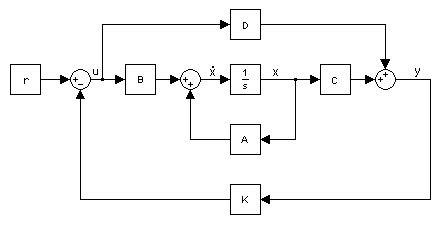
\includegraphics[width=0.7\textwidth]{figures/closed_loop_control.png}
				\end{center}

			\end{column}

			\begin{column}{0.48\textwidth}
				\begin{itemize}
					\item Tracking of reference trajectory
					\item[] \begin{equation}\begin{aligned}
						\dot{x} = Ax + Bu\\
						y = Cx
						\end{aligned}\end{equation}
					\item Only stable systems
				\end{itemize}
			\end{column}
		\end{columns}
	\end{block}
\end{frame}



\begin{frame}{What are we talking about}
	\begin{block}{Use Spiking neural networks}
		\begin{columns}
			\begin{column}{0.48\textwidth}

				\begin{center}
					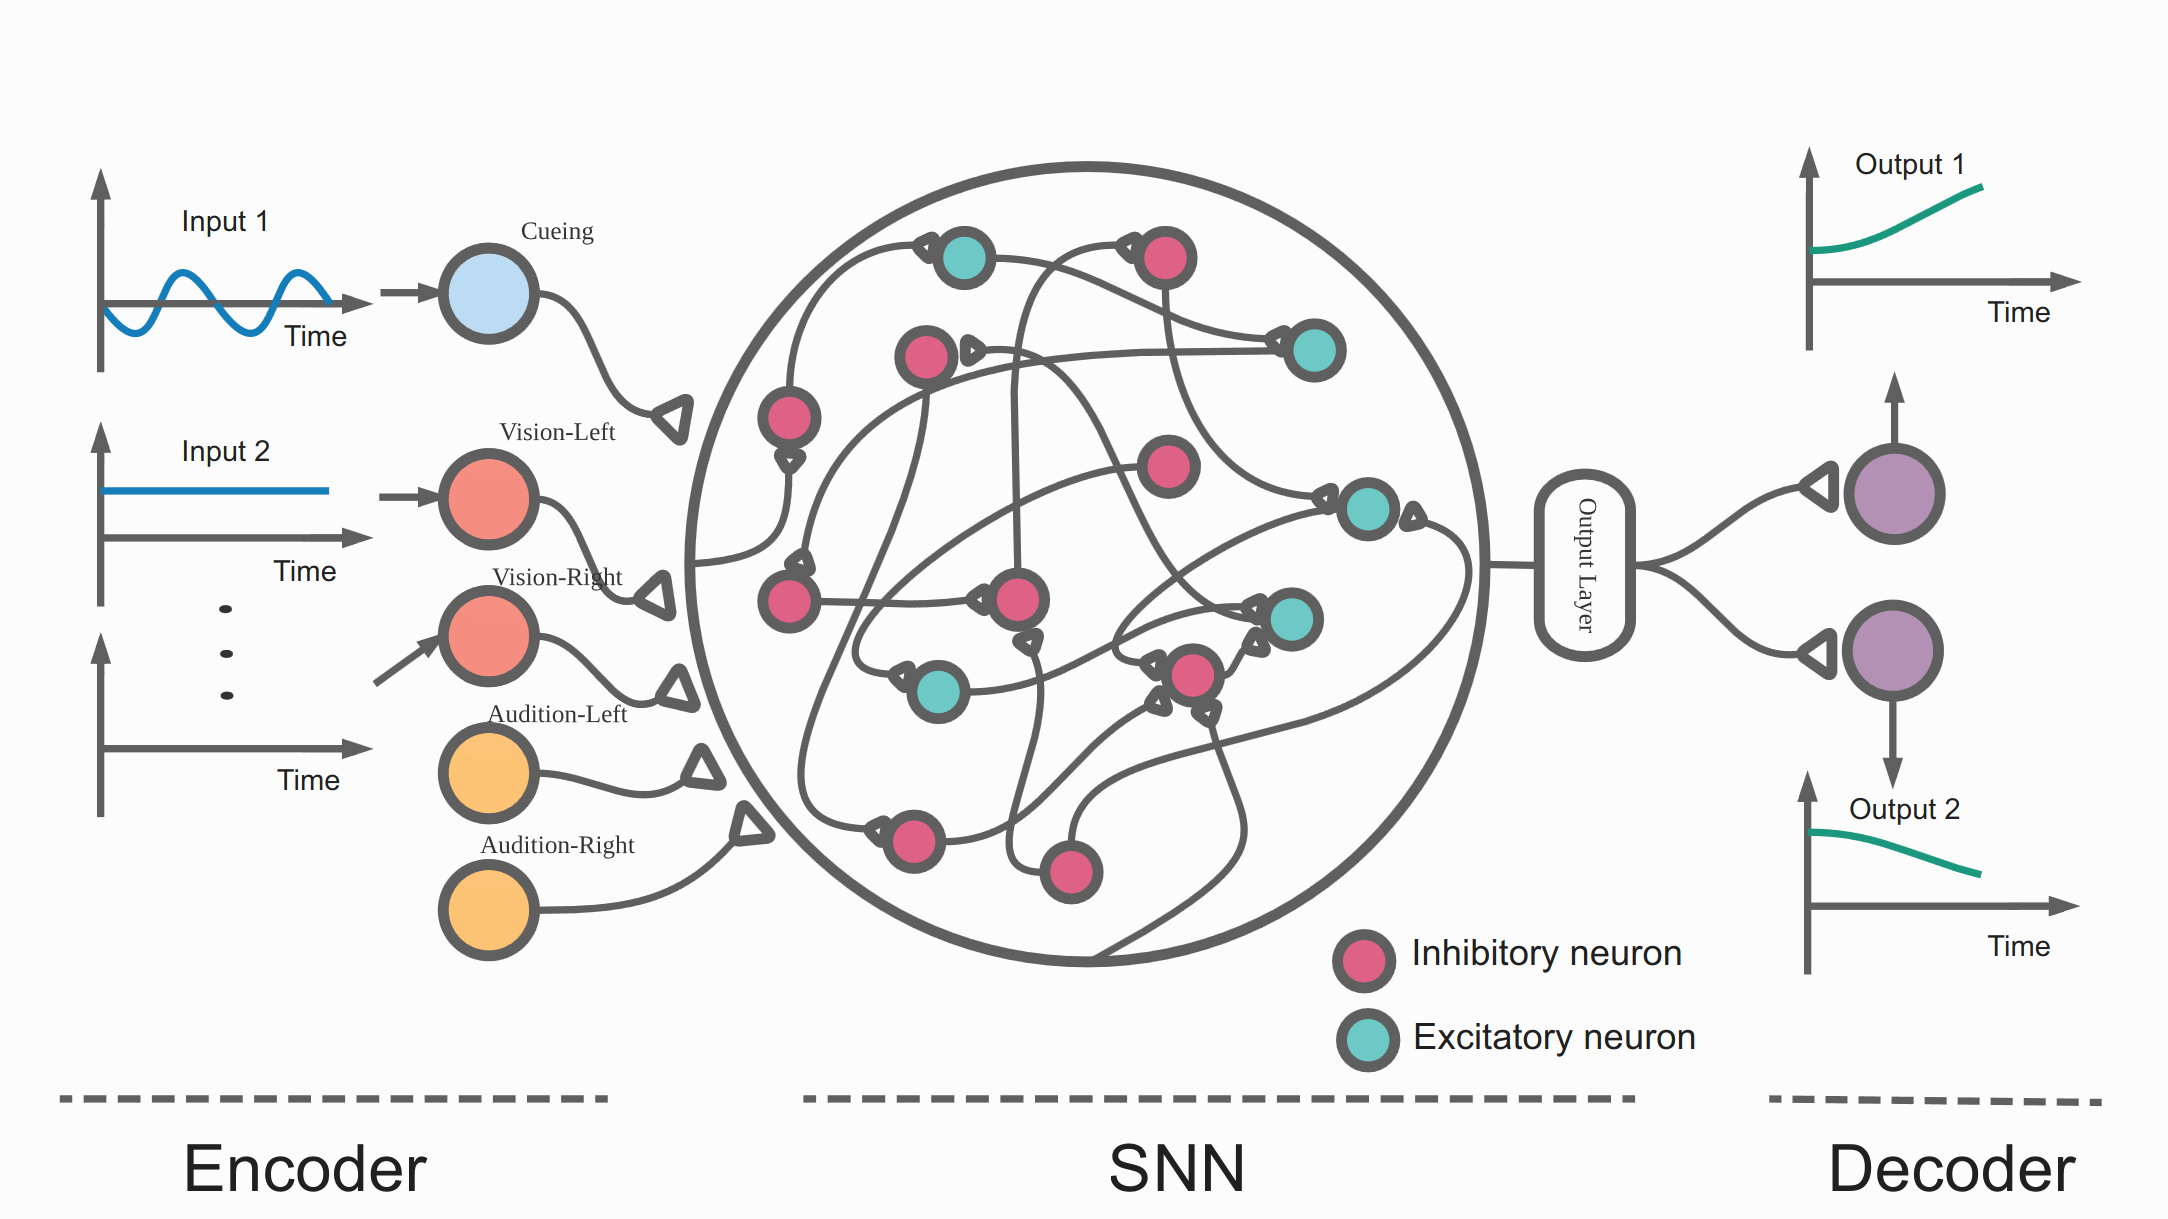
\includegraphics[width=0.7\textwidth]{figures/test.png}
				\end{center}

				\begin{textblock*}{20pt}(250pt,350pt)
					\small
					\cite{Xue2022}
				\end{textblock*}
			\end{column}

			\begin{column}{0.48\textwidth}
				\begin{itemize}
					\setlength\itemsep{1.5em}
					\item Third Generation of NN
					\item Working with discrete spikes
					\item Inherently fit for temporal data
				\end{itemize}
			\end{column}
		\end{columns}
	\end{block}
\end{frame}


\begin{frame}{Method}
	\begin{block}{1. Simulate}
		Use a spiking network to simulate a dynamic system
	\end{block}

	\begin{block}{2. Control}
		Devise a control scheme to control the network output
	\end{block}
	\begin{block}{3. Learn}
		Apply biologically plausible learning rules to our network
	\end{block}

	\begin{block}{4. Combine}
		Integrate all three steps into a single controller
	\end{block}

\end{frame}


\section{Simulation}\insertsectionpage
\begin{frame}{Simulation of Linear systems}
	\begin{columns}[T]
		\begin{column}{0.45\textwidth}
			\begin{figure}
				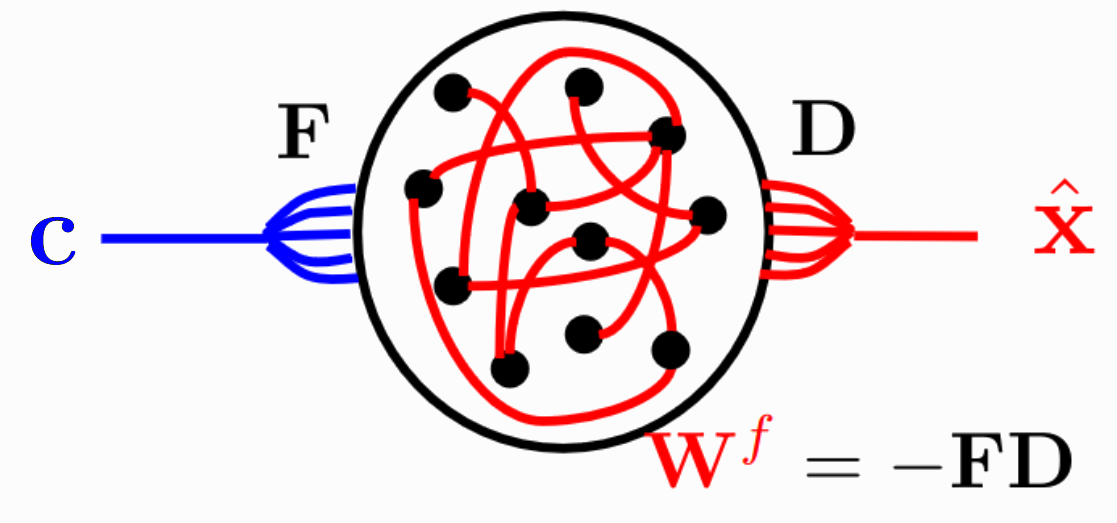
\includegraphics[width=0.9\textwidth]{figures/autoencoder2.png}
			\end{figure}
		\end{column}
		\begin{column}{0.45\textwidth}
			\begin{itemize}
				\item Build NN that outputs $\hat{x}$ from the system $\dot{x} = Ax + c$ given $c$\\
				\item Group of LIF neurons with with intrinsic Voltage, tracking the projected error $V_{i} = F_i(x-\hat{x})+\mu r_{i}$\\
				\item Network decoding $\hat{x} =F^Tr$
			\end{itemize}
		\end{column}
	\end{columns}
	\begin{textblock*}{20pt}(250pt,300pt)
		\begin{equation*}
			\dot{V} = -\lambda_{V}V+Fc+W^{f}o(t)+W^{s}r(t)+\sigma _{V}\eta(t)
		\end{equation*}
	\end{textblock*}

	\begin{textblock*}{20pt}(100pt,250pt)
		\cite{boerlin_predictive_2013}
	\end{textblock*}
\end{frame}


%\begin{frame}{Geometric}
%	\begin{tikzpicture}[remember picture, overlay]
%		\node at (current page.north east) [xshift=-20cm, yshift=-8.85cm] {
%			\begin{tikzpicture}
%				\begin{axis}[
%					width=0.35\textwidth,
%					height=0.35\textwidth,
%					xlabel={$\Delta x$},
%					ylabel={$\Delta y$},
%					xmin =-0.9,
%					xmax = 0.9,
%					ymin = -0.9,
%					ymax = 0.9,
%					axis equal,
%					axis lines=middle,
%					enlargelimits=true,
%					xticklabels ={},
%					yticklabels = {},
%					xlabel style={
%						at={(ticklabel* cs:1.02)}, % Adjust the position of xlabel
%						anchor=north,
%					},
%					ylabel style={
%						at={(ticklabel* cs:1.02)}, % Adjust the position of ylabel
%						anchor=south,
%					},
%					]
%					\draw[->,violet,ultra thick](axis cs:0,0.0)--(axis cs: 0.5,0.5) node[midway,left,text=violet]{$\color{violet} F_1$};
%					\draw[->,teal,ultra thick](axis cs:0,0.0)--(axis cs: -0.5,0.5)node[midway,left,text=violet]{$\color{teal} F_2$};
%					\draw[->,red,ultra thick](axis cs:0,0.0)--(axis cs: 0.5,-0.5)node[midway,right,text=violet]{$\color{red} F_4$};
%					\draw[->,orange,ultra thick](axis cs:0,0.0)--(axis cs: -0.5,-0.5)node[midway,left,text=violet]{$\color{orange} F_3$};
%					\draw[draw = none,top color = white, middle color = white,bottom color = violet,shading angle = -90,opacity = 0.6,transform canvas = {rotate around={45:(axis cs: 0.0,0.0)}}] (axis cs:0.707,-5) rectangle (axis cs:0.9,5);
%					\draw[draw = none,top color = white, middle color = white,bottom color = teal,shading angle = -90,opacity = 0.6,transform canvas = {rotate around={135:(axis cs: 0.0,0.0)}}] (axis cs:0.707,-5) rectangle (axis cs:0.9,5);
%					\draw[draw = none,top color = white, middle color = white,bottom color = orange,shading angle = -90,opacity = 0.6,transform canvas = {rotate around={225:(axis cs: 0.0,0.0)}}] (axis cs:0.707,-5) rectangle (axis cs:0.9,5);
%					\draw[draw = none,top color = white, middle color = white,bottom color = red,shading angle = -90,opacity = 0.6,transform canvas = {rotate around={-45:(axis cs: 0.0,0.0)}}] (axis cs:0.707,-5) rectangle (axis cs:0.9,5);
%
%				\end{axis}
%		\end{tikzpicture}};
%	\end{tikzpicture}
%
%	\begin{tikzpicture}[remember picture, overlay]
%		\node at (current page.north east) [xshift=-8cm, yshift=-7.5cm] {
%			\begin{tikzpicture}
%				\begin{axis}[
%					width=0.5\textwidth,
%					height=0.3\textwidth,
%					xlabel={$x$},
%					ylabel={$y$},
%					domain=0:3.5,
%					samples=100,
%					axis lines=middle,
%					enlargelimits=true,
%					clip mode=individual, % Ensure everything is shown
%					xticklabels ={},
%					yticklabels = {},
%					xlabel style={
%						at={(ticklabel* cs:0.5)}, % Adjust the position of xlabel
%						anchor=north,
%					},
%					ylabel style={
%						at={(ticklabel* cs:0.5)}, % Adjust the position of ylabel
%						anchor=south,
%						rotate=90, % Rotate ylabel by 90 degrees
%					},
%					]
%					\addplot[blue,thick] {0.28934*x^3 - 1.8178*x^2 + 2.6016*x^1 + 0.66431};
%					\draw[->,violet,ultra thick](axis cs:0,0.66)--(axis cs: 0.353553,1.01355);
%					\draw[->,teal,ultra thick](axis cs:0.353553,1.01355)--(axis cs: 5.55112e-17,1.36711);
%					\draw[->,violet,ultra thick](axis cs:5.55112e-17,1.36711)--(axis cs: 0.353553,1.72066);
%					\draw[->,red,ultra thick](axis cs:0.353553,1.72066)--(axis cs: 0.707107,1.36711);
%					\draw[->,violet,ultra thick](axis cs:0.707107,1.36711)--(axis cs: 1.06066,1.72066);
%					\draw[->,red,ultra thick](axis cs:1.06066,1.72066)--(axis cs: 1.41421,1.36711);
%					\draw[->,red,ultra thick](axis cs:1.41421,1.36711)--(axis cs: 1.76777,1.01355);
%					\draw[->,red,ultra thick](axis cs:1.76777,1.01355)--(axis cs: 2.12132,0.66);
%					\draw[->,red,ultra thick](axis cs:2.12132,0.66)--(axis cs: 2.47487,0.306447);
%					\draw[->,red,ultra thick](axis cs:2.47487,0.306447)--(axis cs: 2.82843,-0.0471068);
%					\draw[->,red,ultra thick](axis cs:2.82843,-0.0471068)--(axis cs: 3.18198,-0.40066);
%					\draw[->,violet,ultra thick](axis cs:3.18198,-0.40066)--(axis cs: 3.53553,-0.0471068);
%				\end{axis}
%		\end{tikzpicture}};
%	\end{tikzpicture}
%\end{frame}



\begin{frame}{Example Simulation}
	\begin{textblock*}{5cm}(50pt,150pt)
		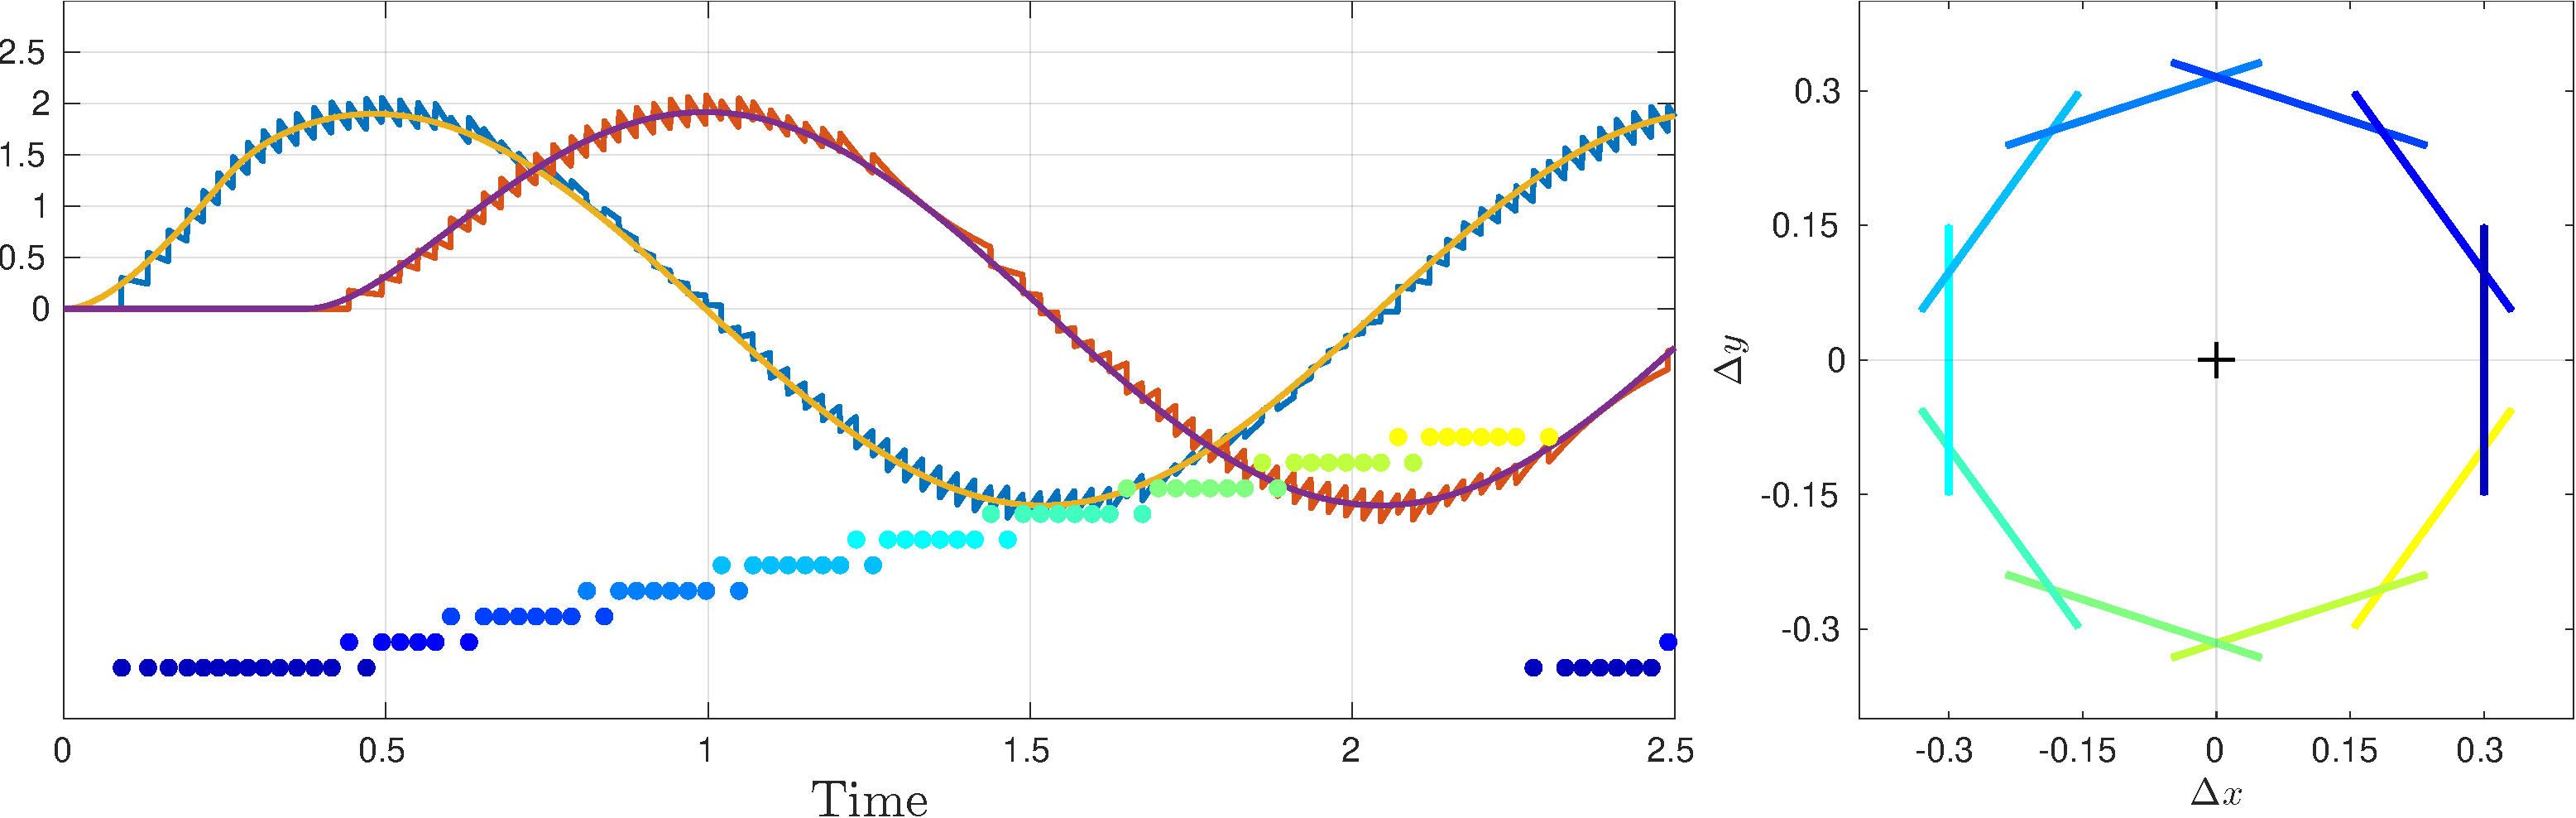
\includegraphics[scale= 0.4]{figures/plots/Simulation/2d_perfect_gamma.pdf}
	\end{textblock*}
\end{frame}



\section{Control}\insertsectionpage
\begin{frame}{Control Concept}
	\vspace{-0.3cm}
	\begin{center}
		\begin{tikzpicture}
			% Include the picture
			\node[anchor=south west, inner sep=0] (image) at (100pt,100pt) {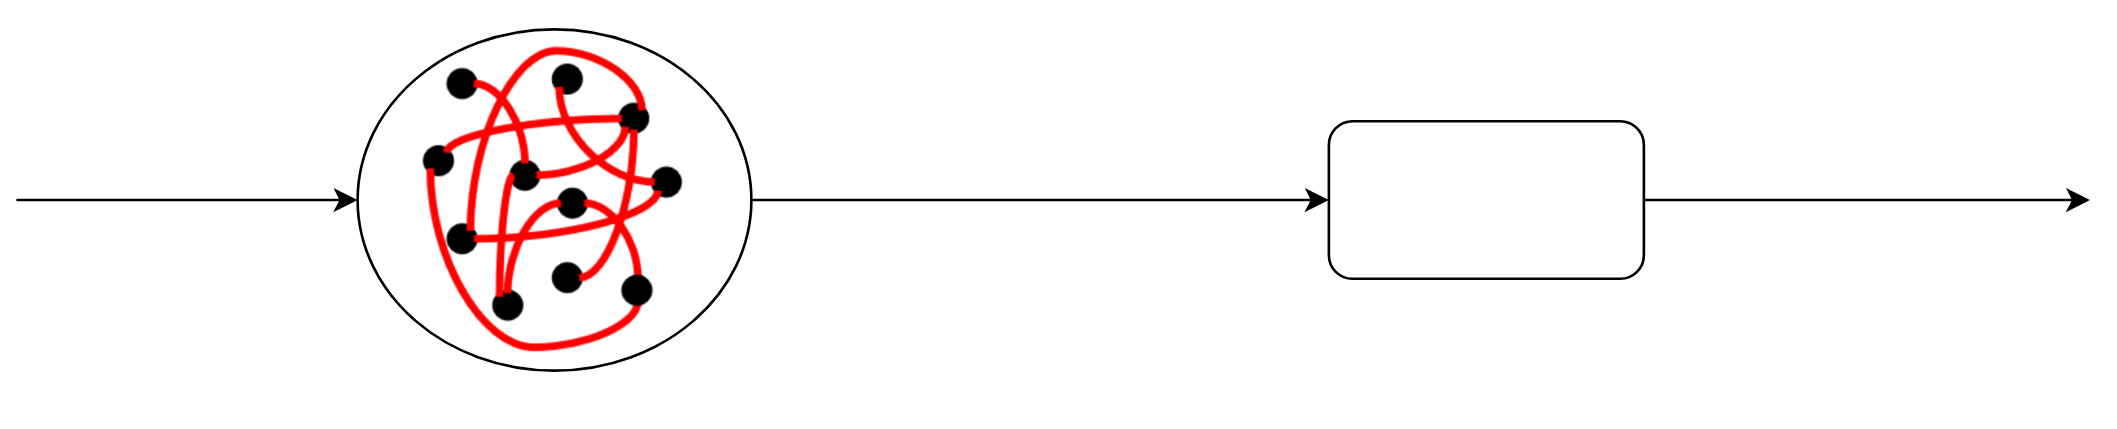
\includegraphics[width=0.7\textwidth]{figures/control_1.png}};

			% Overlay equation
			\node[anchor=south west, align=left, opacity=1] at ([shift={(288pt,25pt)}]image.south west)  {\scalebox{0.7}{$
					\begin{aligned}
						\dot{x} &= Ax + Bu\\
						y &= Cx
					\end{aligned}
					$}};

			\node[anchor=south west, align=left, opacity=1] at ([shift={(380pt,50pt)}]image.south west)  {\scalebox{0.7}{$\hat{x}$}};
			\node[anchor=south west, align=left, opacity=1] at ([shift={(210pt,50pt)}]image.south west)  {\scalebox{0.7}{$u$}};
			\node[anchor=south west, align=left, opacity=1] at ([shift={(30pt,50pt)}]image.south west)  {\scalebox{0.7}{$\text{x}$}};
		\end{tikzpicture}
	\end{center}
	\begin{textblock*}{50pt}(650pt,180pt)
		\small
		\cite{huang_spiking_2019}
	\end{textblock*}
 	\vspace{-0.3cm}
	\begin{itemize}
		\item (Almost) identical network architecture
		\item Network output is external input into (previous) simulating network
		$\longleftrightarrow$ Network state contains control signal
		\item Governed by PD-control as $c= \dot{x}-Ax$
		\item In presence of output matrix $C\neq \mathbf{I} \leftrightarrow \rank(B^TC^T) = rank(B^T)$
	\end{itemize}

\end{frame}


\begin{frame}{Example}

	\begin{figure}
		\centering
		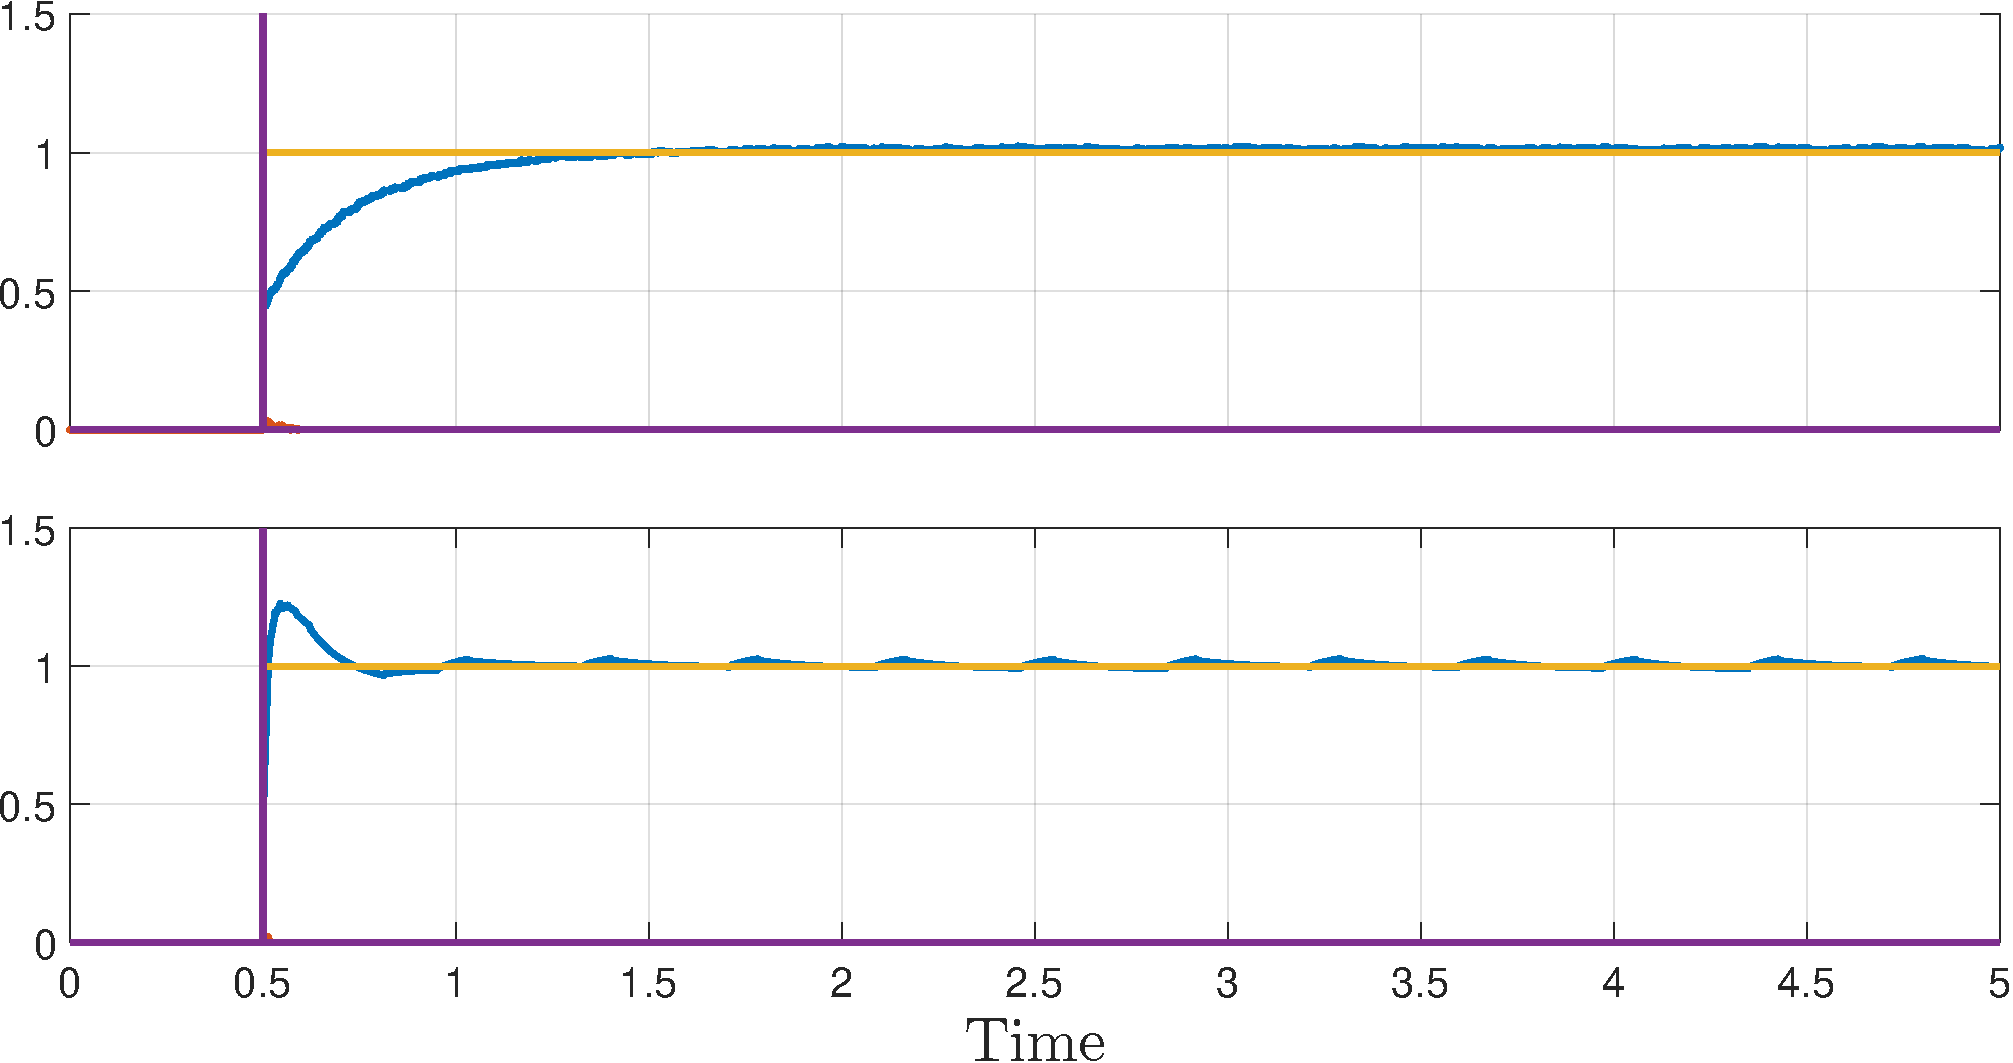
\includegraphics[scale = 0.45]{figures/plots/Control/compare_step_both_methods.pdf}
	\end{figure}
\end{frame}


\section{Learning}\insertsectionpage

\begin{frame}{Learning rules \cite{bourdoukan_enforcing_2015}}

	\begin{textblock*}{20pt}(550pt,50pt)
		\begin{equation*}
			V_i = F_i(x-\hat{x}) - \mu r_i
		\end{equation*}
	\end{textblock*}

	\begin{columns}
		\begin{column}{0.45\textwidth}
			\textbf{Slow Learning rule} $W^s = F(A+\lambda_d\mathbf{I})F^T$
			\begin{itemize}
				\item Online Learning of Student teacher dynamics $\dot{\hat{x}} = M\hat{x} +c$
				\item Error Feedback $e$ during Training
				\item $\delta M \propto e\hat{x}^T \longrightarrow \delta W^s \propto F(e\hat{x}^T)F^T \approx Fer^T$
				\item Supervised Learning rule
			\end{itemize}

		\end{column}
		\begin{column}{0.45\textwidth}
			\textbf{Fast Learning rule} $W^f = FF^T + \mu\mathbf{I}$
			\begin{itemize}
				\item Voltage measures system error
				\item Minimize average Voltage outside of Neuron Threshold
				\item Biologically plausible $\text{pre}\times\text{post}$ locally
				\item Unsupervised Learning Rule
			\end{itemize}
		\end{column}
	\end{columns}
\end{frame}


\begin{frame}{Example}
	\begin{figure}
		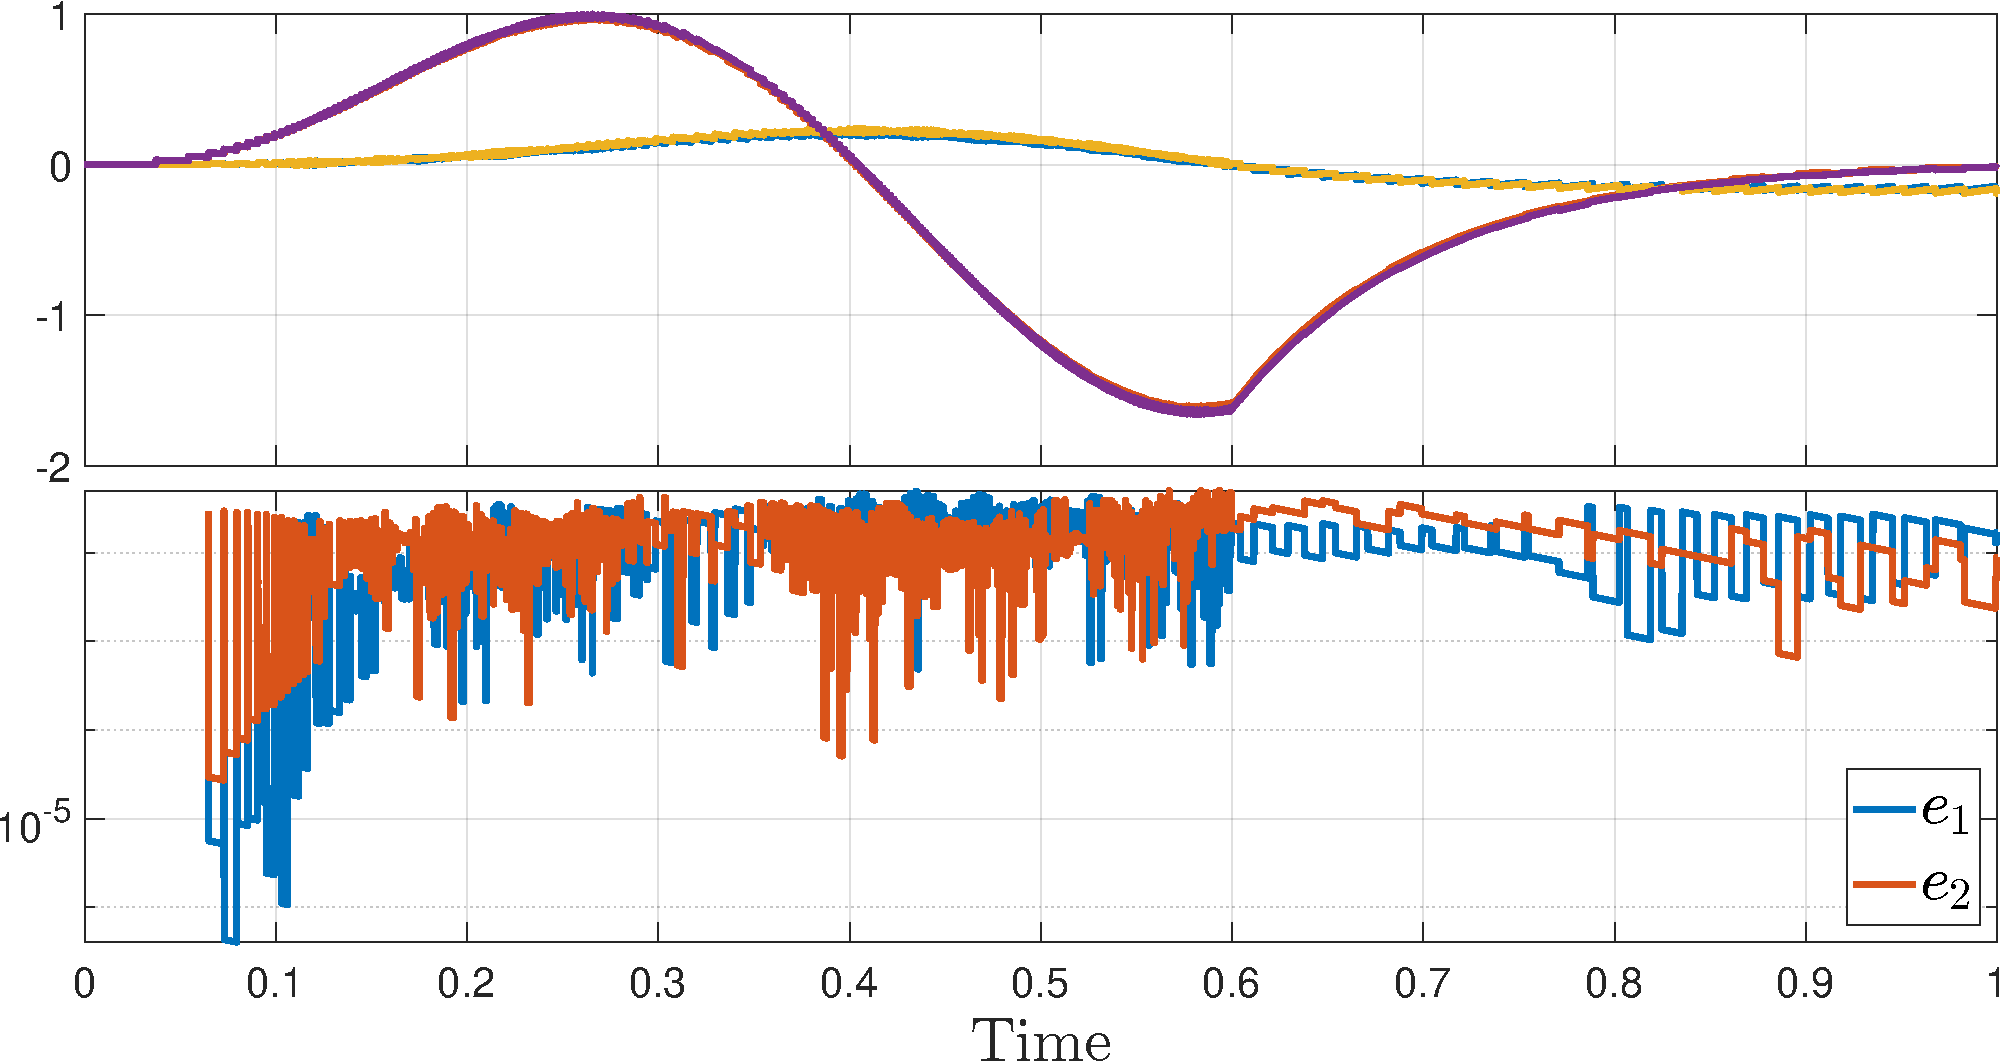
\includegraphics[scale = 0.45]{figures/plots/Learning/error_compare.pdf}
	\end{figure}
\end{frame}


\section{Combined Learning}\insertsectionpage

\begin{frame}{Control Concept}
	\vspace{-0.7cm}
	\begin{center}
		\begin{tikzpicture}
			% Include the picture
			\node[anchor=south west, inner sep=0] (image) at (100pt,100pt) {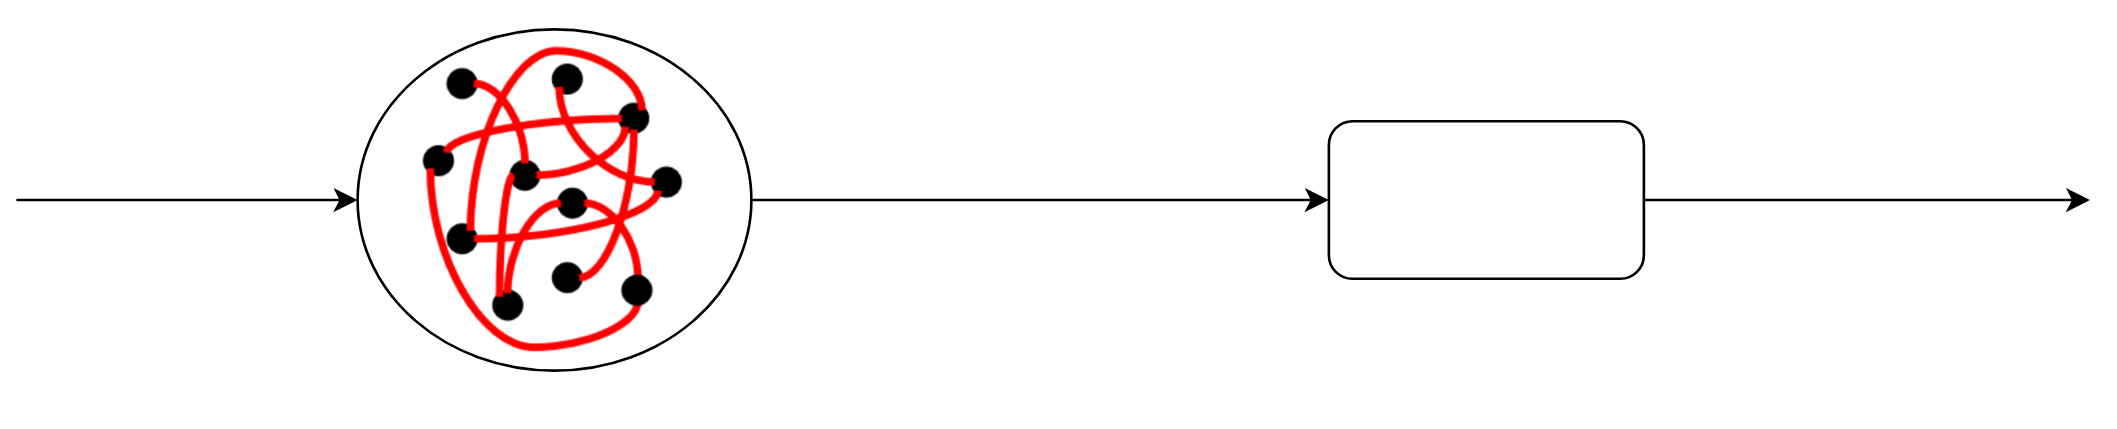
\includegraphics[width=0.7\textwidth]{figures/control_1.png}};

			% Overlay equation
			\node[anchor=south west, align=left, opacity=1] at ([shift={(288pt,25pt)}]image.south west)  {\scalebox{0.7}{$
					\begin{aligned}
						\dot{x} &= Ax + Bu\\
						y &= Cx
					\end{aligned}
					$}};

			\node[anchor=south west, align=left, opacity=1] at ([shift={(380pt,50pt)}]image.south west)  {\scalebox{0.7}{$\hat{x}$}};
			\node[anchor=south west, align=left, opacity=1] at ([shift={(210pt,50pt)}]image.south west)  {\scalebox{0.7}{$c$}};
			\node[anchor=south west, align=left, opacity=1] at ([shift={(30pt,50pt)}]image.south west)  {\scalebox{0.7}{$\text{x}$}};
		\end{tikzpicture}
	\end{center}
	\pause
	\vspace{-0.9cm}
	\begin{center}
		\begin{tikzpicture}
			% Include the picture
			\node[anchor=south west, inner sep=0] (image) at (100pt,100pt) {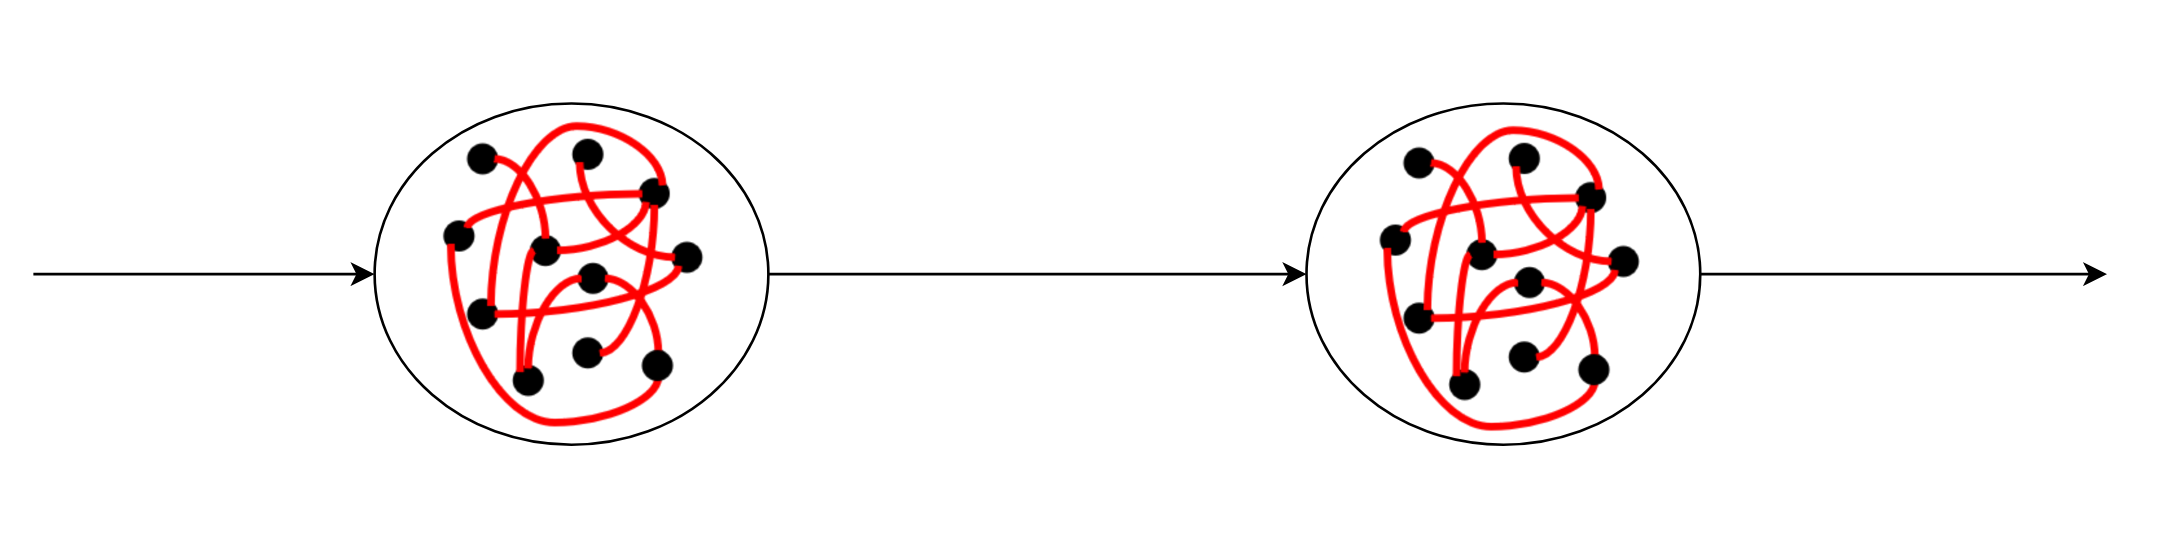
\includegraphics[width=0.7\textwidth]{figures/control_2.png}};

			\node[anchor=south west, align=left, opacity=1] at ([shift={(380pt,60pt)}]image.south west)  {\scalebox{0.7}{$\hat{x}$}};
			\node[anchor=south west, align=left, opacity=1] at ([shift={(210pt,60pt)}]image.south west)  {\scalebox{0.7}{$c$}};
			\node[anchor=south west, align=left, opacity=1] at ([shift={(30pt,60pt)}]image.south west)  {\scalebox{0.7}{$\text{x}$}};
		\end{tikzpicture}

	\end{center}
	\begin{textblock*}{50pt}(650pt,180pt)
		\small
		\cite{huang_spiking_2019}
	\end{textblock*}
	\pause
	\vspace{-1.3cm}
	\begin{center}
		\begin{tikzpicture}
			% Include the picture
			\node[anchor=south west, inner sep=0] (image) at (100pt,100pt) {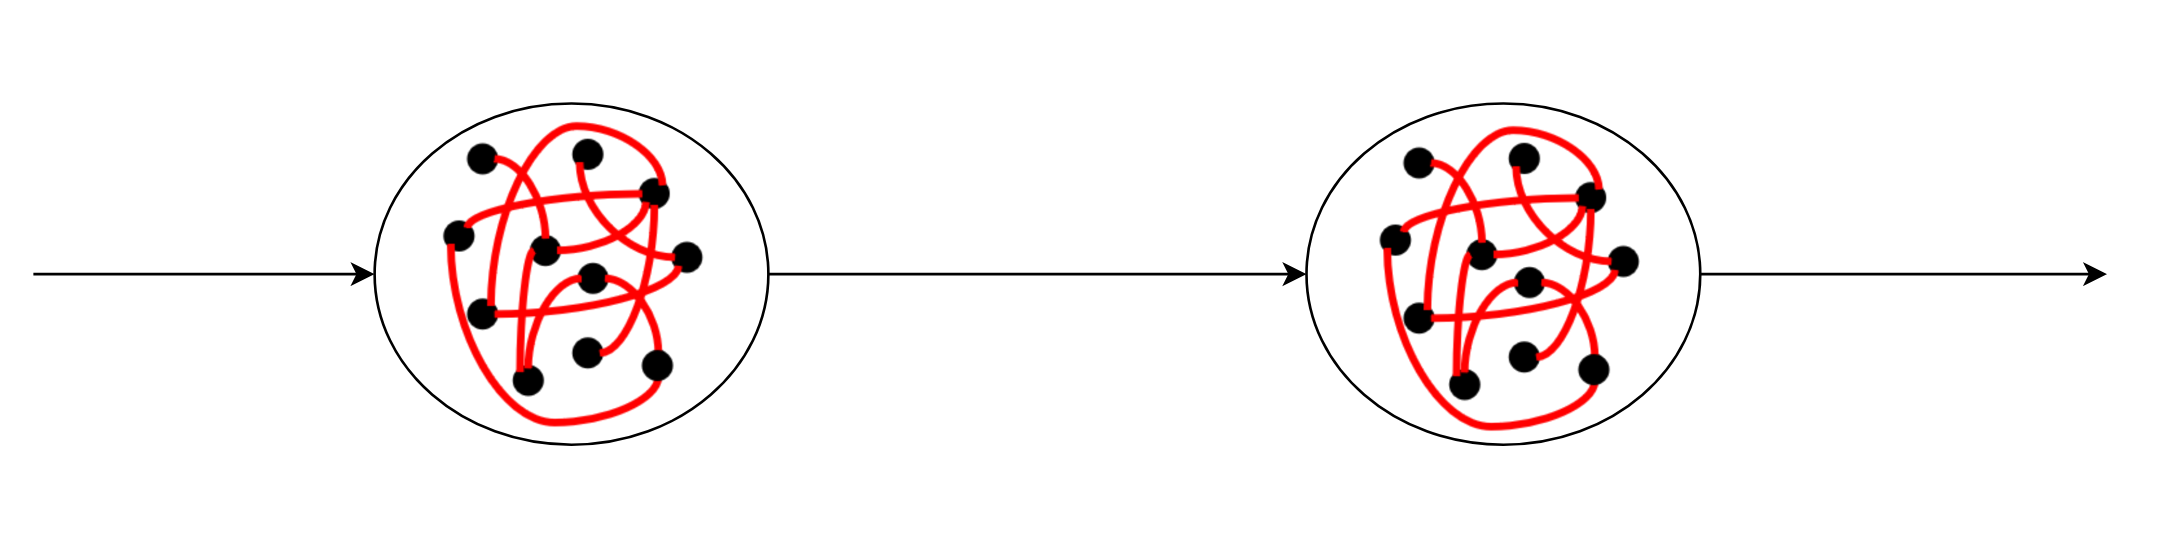
\includegraphics[width=0.7\textwidth]{figures/control_2.png}};

			\node[anchor=south west, align=left, opacity=1] at ([shift={(380pt,60pt)}]image.south west)  {\scalebox{0.7}{$\hat{x}$}};
			\node[anchor=south west, align=left, opacity=1] at ([shift={(210pt,60pt)}]image.south west)  {\scalebox{0.7}{$c$}};
			\node[anchor=south west, align=left, opacity=1] at ([shift={(30pt,60pt)}]image.south west)  {\scalebox{0.7}{$\text{x}$}};

			\node[] at ([shift={(160pt,60pt)}]image.south west) (A) {};
			\node[] at ([shift={(145pt,80pt)}]image.south west) (B) {};
			\draw[thick,blue, ->] ([shift={(160pt,70pt)}]image.south west) arc (-70:145:0.3cm);% syntax (starting point coordinates) arc (starting angle:ending angle:radius)
			\draw[thick,blue, ->] ([shift={(358pt,70pt)}]image.south west) arc (-70:145:0.3cm);% syntax (starting point coordinates) arc (starting angle:ending angle:radius)

		\end{tikzpicture}

	\end{center}



\end{frame}


\begin{frame}{Problems}
	In conjunction, problems can arise:\\
	\begin{itemize}
		\setlength\itemsep{1.0em}
		\item Divergence in Learning
		\item Open loop control
		\begin{itemize}
			\item Noise detection or correction
			\item Compensation of Training errors
		\end{itemize}
		\item High dependence on governing dynamics $c_{ref} =  \dot{x}_\text{ref}- Ax_{ref}$
		\item Orthonormality restriction on Input Matrix $B \in \mathbb{B} := \left\{M\ |\ MM^T = \mathbf{I}\right\}$
		\item No biologically plausible Learning rule for control network available
	\end{itemize}
\end{frame}




\begin{frame}{Control Concept II}


	\begin{textblock*}{50pt}(400pt,270pt)
		\scalebox{0.12}[0.12]{
			\begin{tikzpicture}
				% Include the picture
				\node[anchor=south west, inner sep=0] (image) at (0pt,0pt) {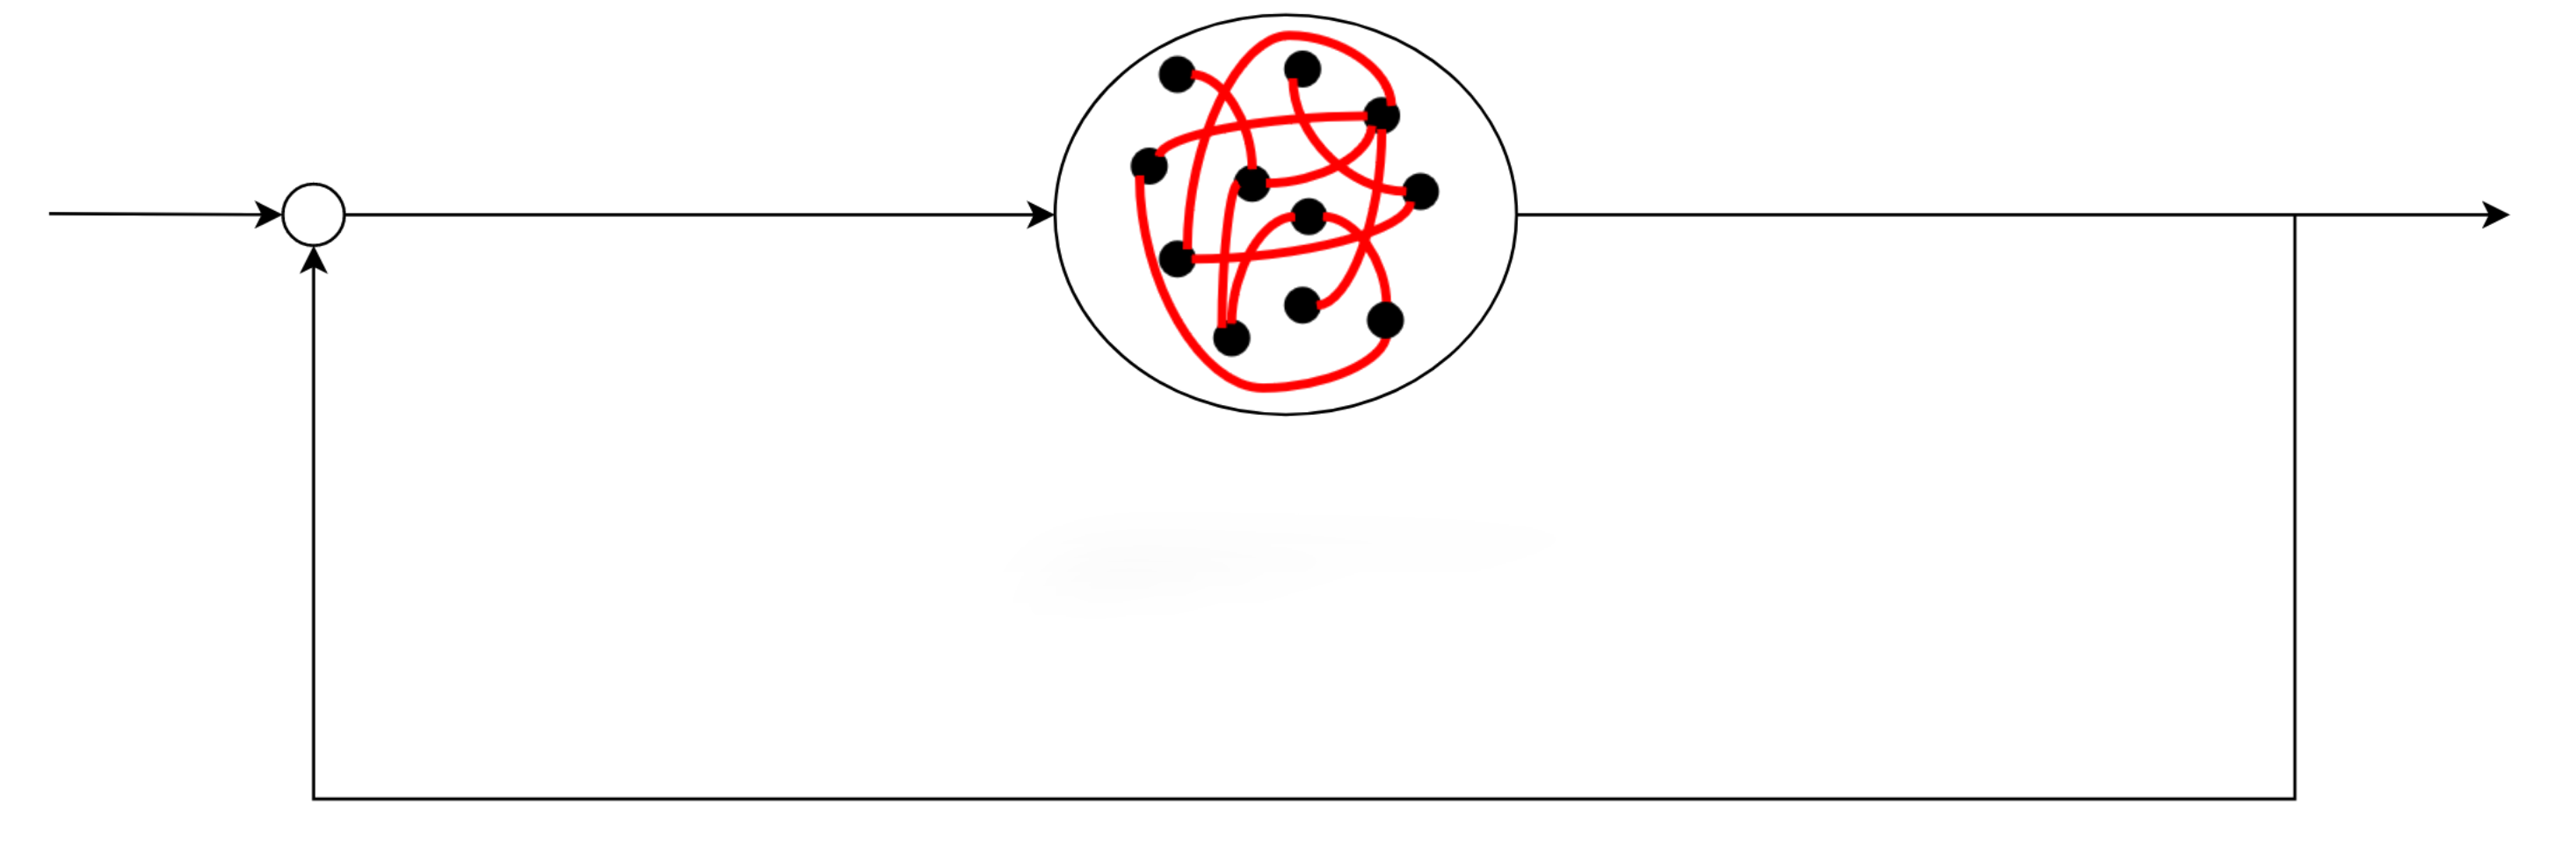
\includegraphics{figures/control_4.png}};
			\end{tikzpicture}
		}
	\end{textblock*}


	\begin{textblock*}{50pt}(410pt,145pt)
		\scalebox{0.15}[0.15]{
			\begin{tikzpicture}
				% Include the picture
				\node[anchor=south west, inner sep=0] (image) at (0pt,0pt) {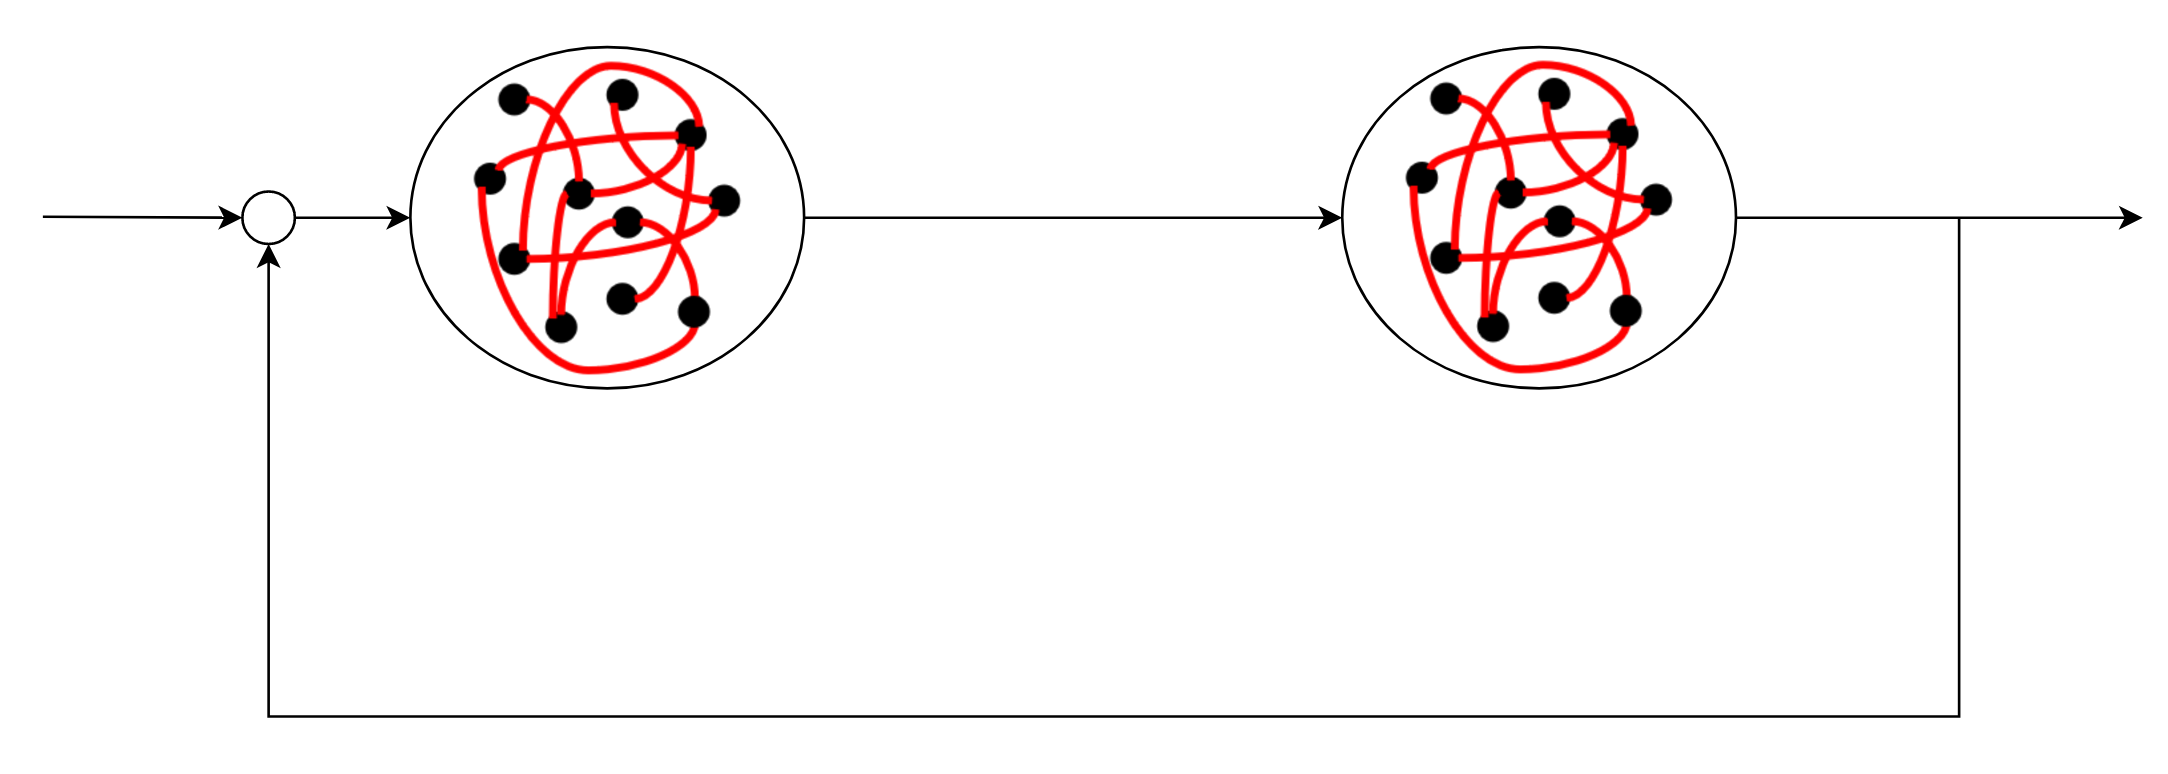
\includegraphics{figures/control_3.png}};
			\end{tikzpicture}
		}
	\end{textblock*}


	\begin{textblock*}{50pt}(70pt,260pt)
		\scalebox{0.15}[0.15]{
			\begin{tikzpicture}
				% Include the picture
				\node[anchor=south west, inner sep=0] (image) at (0pt,0pt) {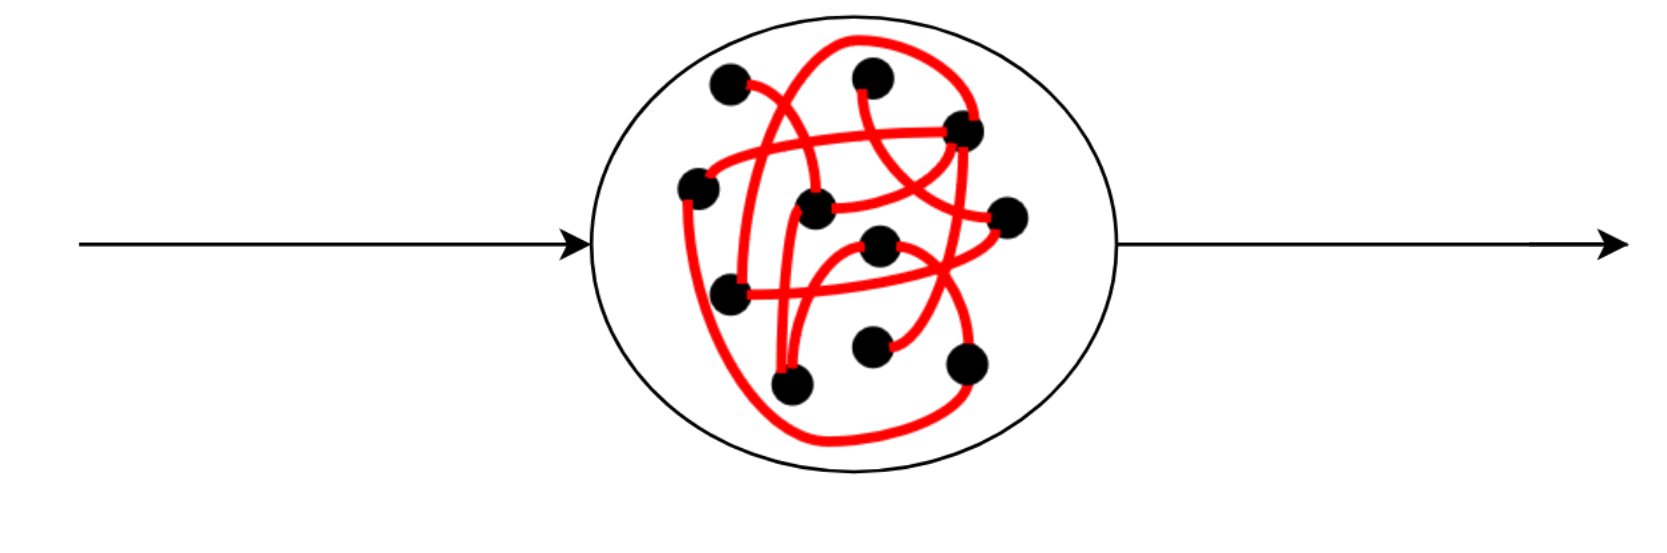
\includegraphics{figures/control_5.png}};
			\end{tikzpicture}
		}
	\end{textblock*}


	\begin{textblock*}{50pt}(50pt,140pt)
	\scalebox{0.15}[0.15]{
		\begin{tikzpicture}
			% Include the picture
			\node[anchor=south west, inner sep=0] (image) at (0pt,0pt) {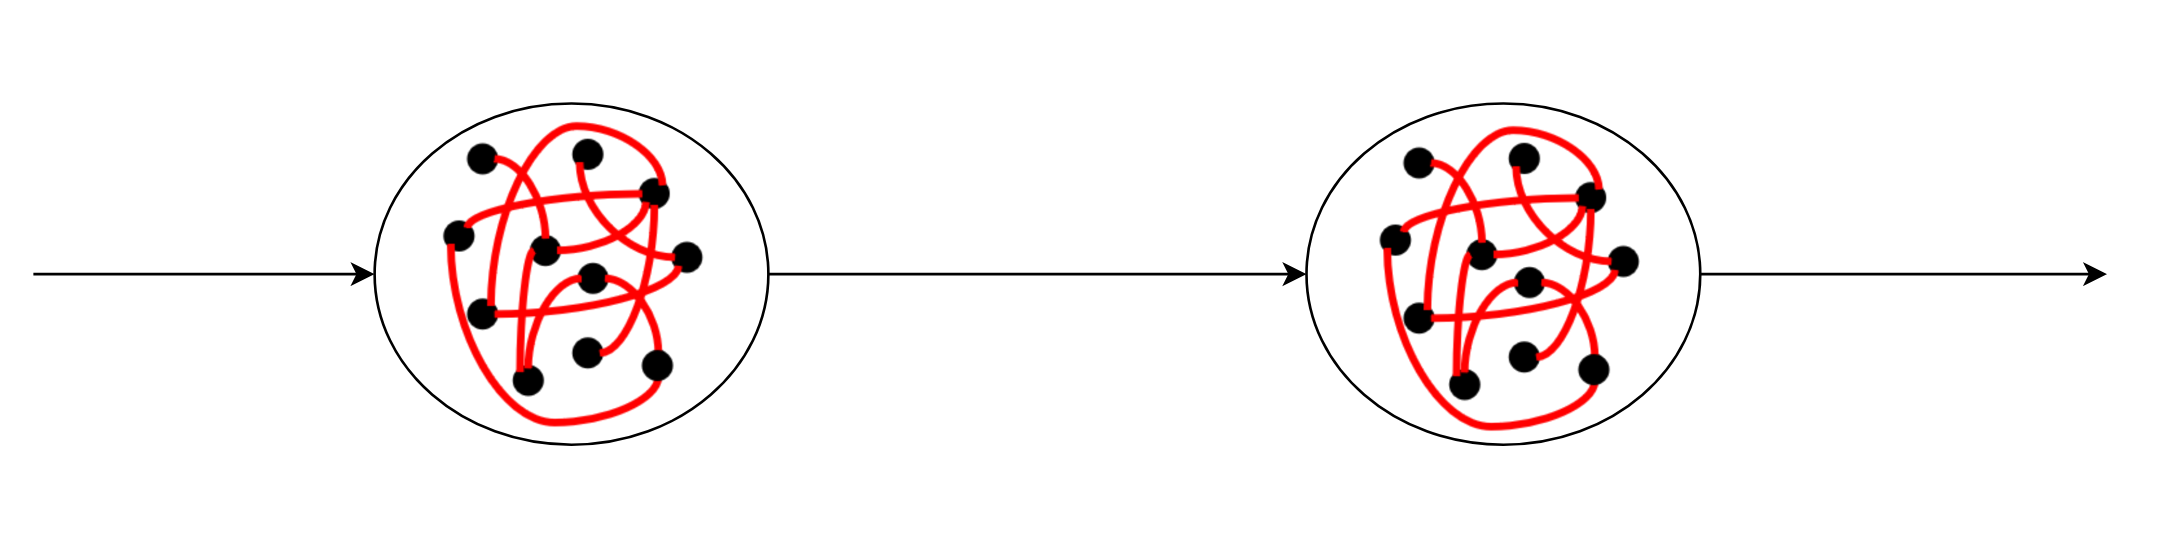
\includegraphics{figures/control_2.png}};
		\end{tikzpicture}
	}
	\end{textblock*}

\end{frame}



\begin{frame}{Summary}
	\begin{textblock*}{50pt}(147pt,119pt)
		\scalebox{0.1}[0.1]{
			\begin{tikzpicture}[]
			% Include the picture
			\node[anchor=south west, inner sep=0] (image) at (0pt,0pt) {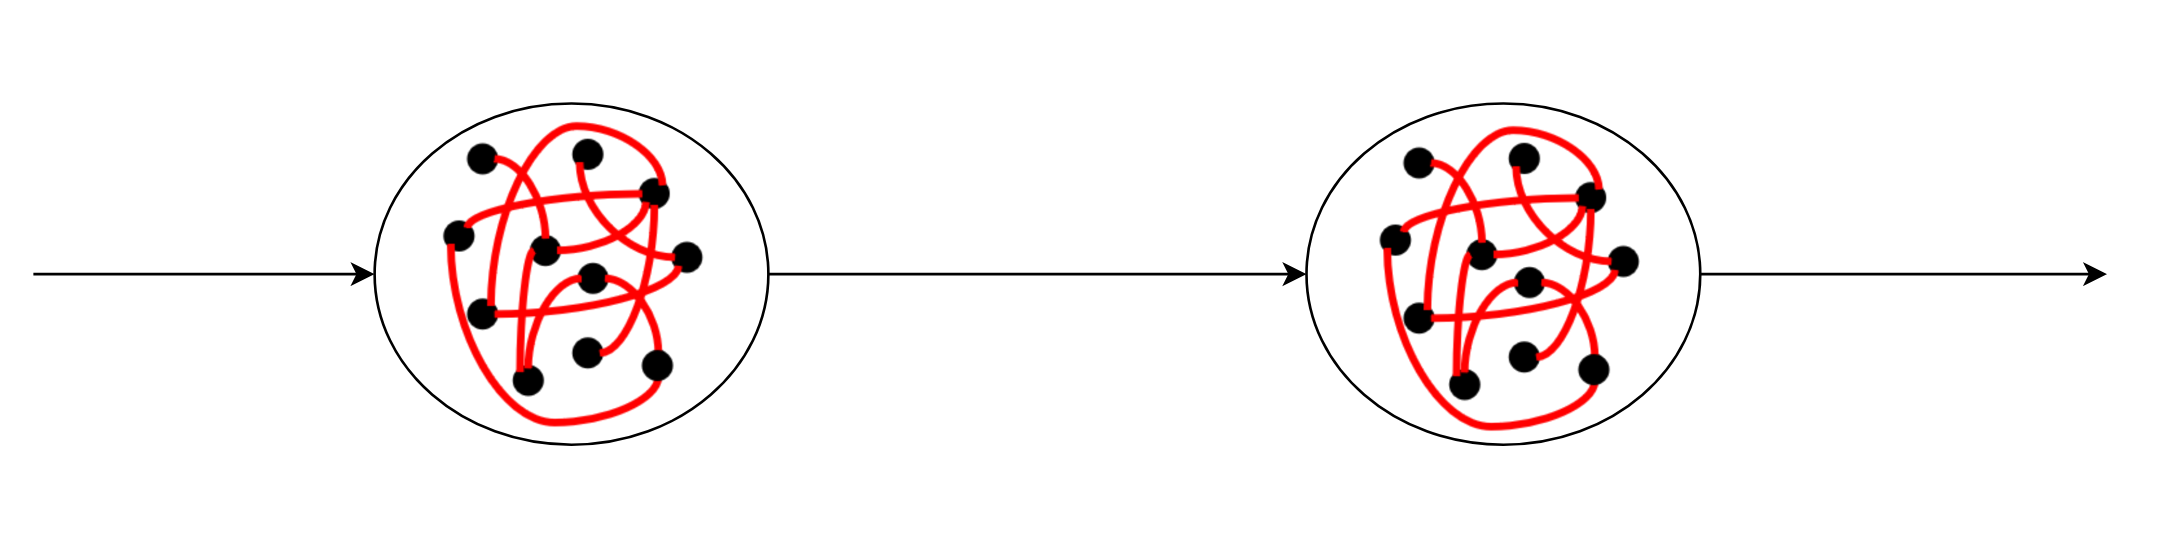
\includegraphics{figures/control_2.png}};
			\end{tikzpicture}}
	\end{textblock*}

	\begin{textblock*}{50pt}(290pt,115pt)
		\scalebox{0.09}[0.09]{
			\begin{tikzpicture}[]
			% Include the picture
			\node[anchor=south west, inner sep=0] (image) at (0pt,0pt) {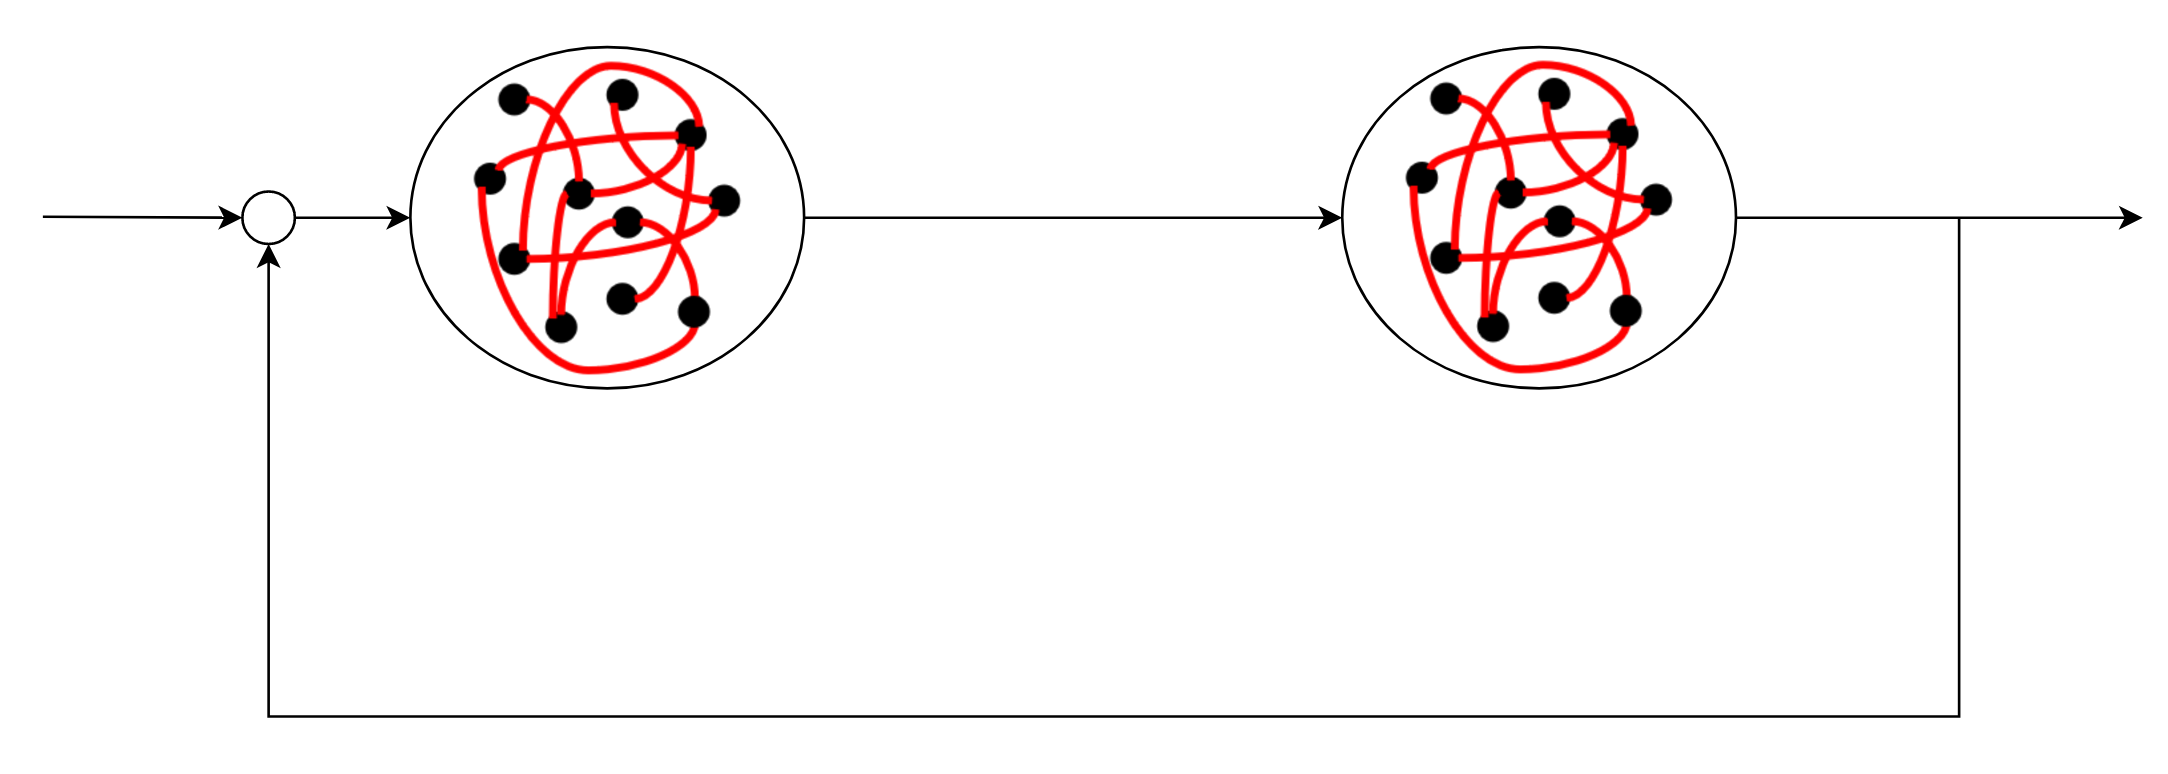
\includegraphics{figures/control_3.png}};
			\end{tikzpicture}}
	\end{textblock*}

	\begin{textblock*}{50pt}(435pt,111pt)
		\scalebox{0.1}[0.1]{
			\begin{tikzpicture}[]
			% Include the picture
			\node[anchor=south west, inner sep=0] (image) at (0pt,0pt) {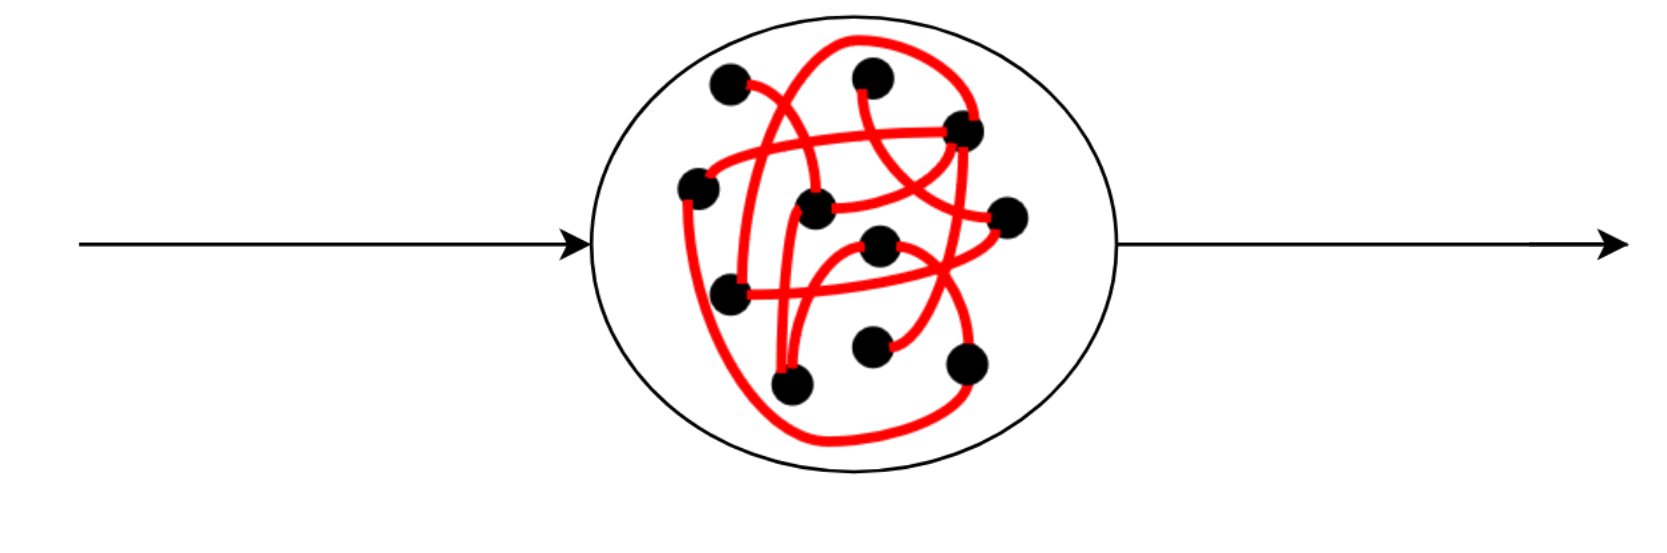
\includegraphics{figures/control_5.png}};
			\end{tikzpicture}}
	\end{textblock*}

	\begin{textblock*}{50pt}(555pt,117pt)
		\scalebox{0.07}[0.07]{
			\begin{tikzpicture}[]
			% Include the picture
			\node[anchor=south west, inner sep=0] (image) at (0pt,0pt) {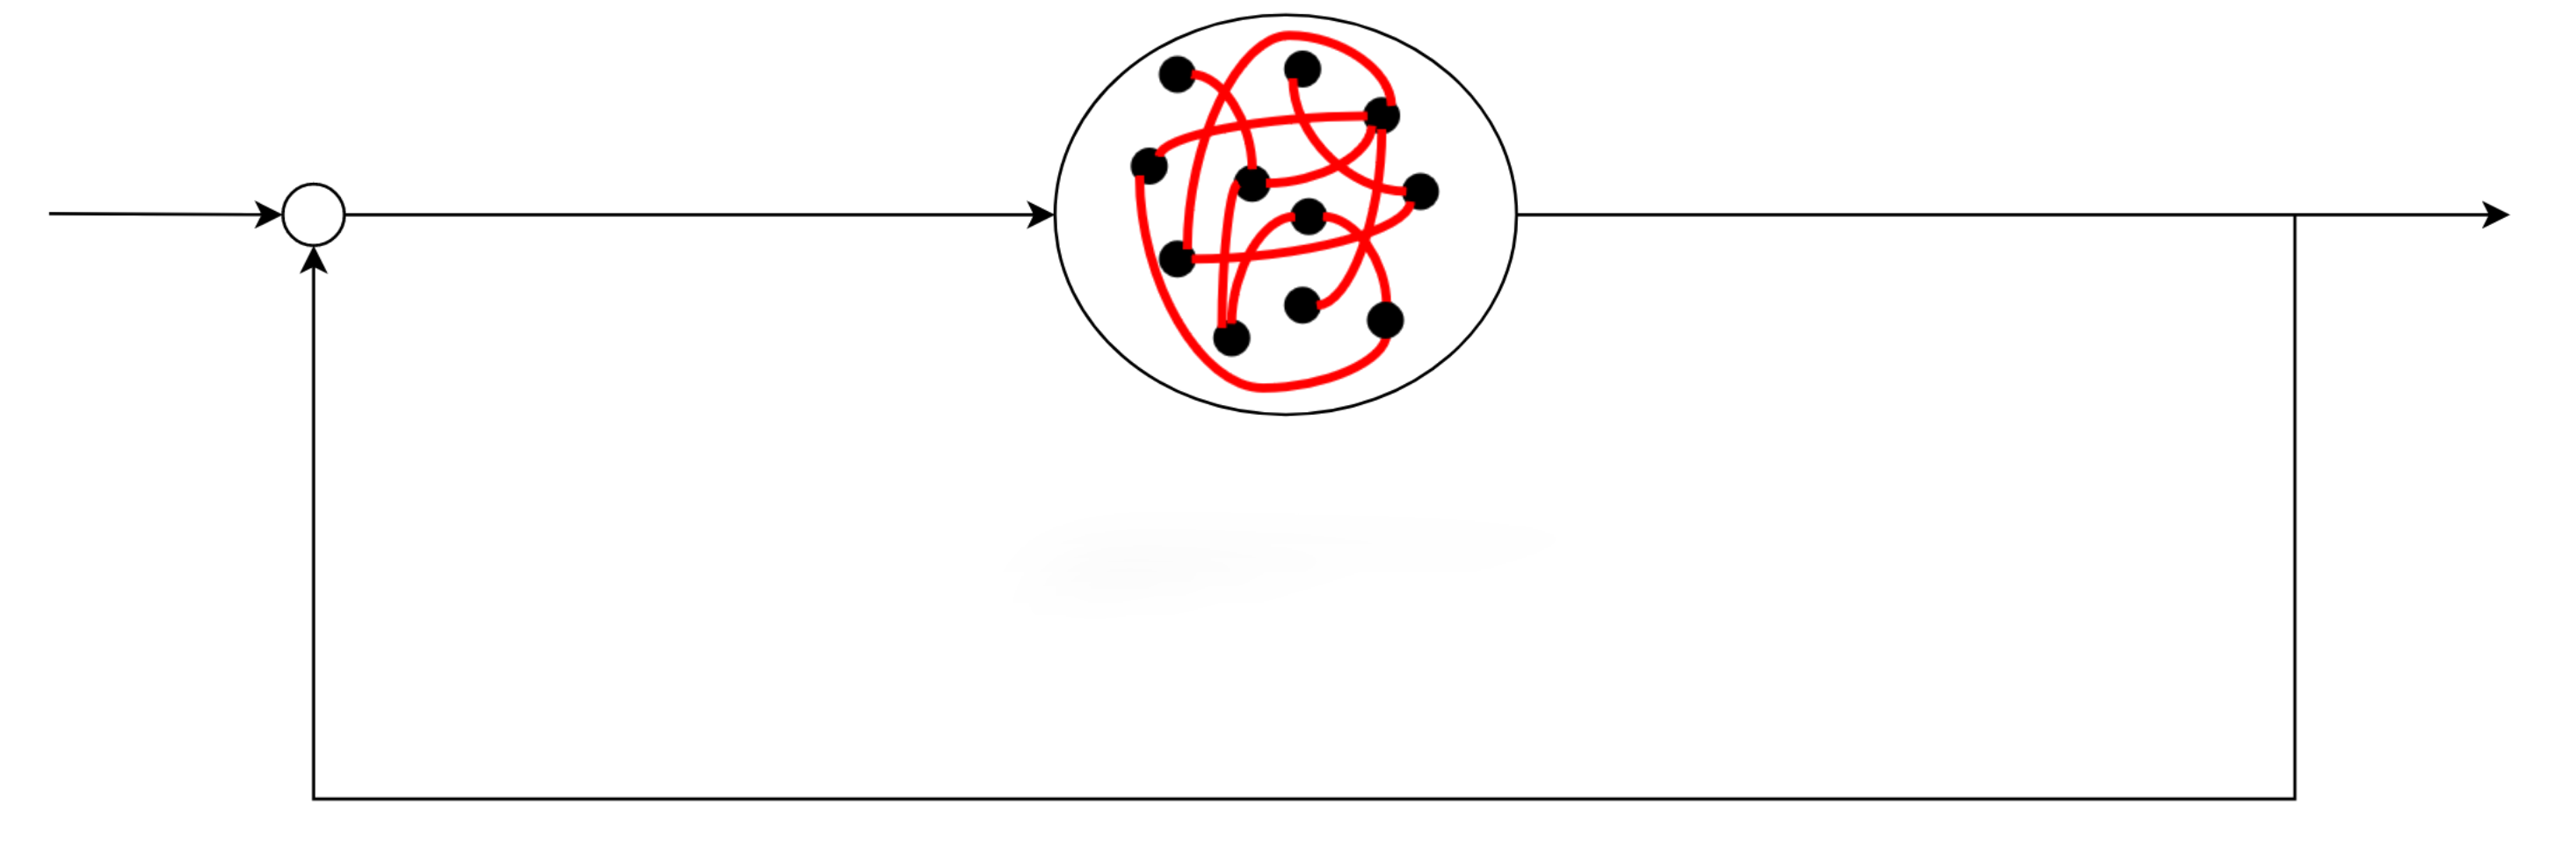
\includegraphics{figures/control_4.png}};
			\end{tikzpicture}}
	\end{textblock*}

	\vspace{1.5cm}
	\begin{table}
		\centering
		\begin{tabular}{ L{4.15cm} | C{4.3cm} | C{4.3cm} | C{4.3cm} | C{4.0cm}}
			High $c_\text{ref}$ dependence & \cellcolor{green!25} Yes & \cellcolor{red!25}No & \cellcolor{green!25} Yes & \cellcolor{red!25}No\\
			\hline
			Open loop control& \cellcolor{green!25} Yes & \cellcolor{red!25}No & \cellcolor{green!25} Yes & \cellcolor{red!25}No\\
			\hline
			Implausible $B$ learning rule & \cellcolor{green!25} Yes & \cellcolor{green!25} Yes & \cellcolor{red!25}No & \cellcolor{red!25}No\\
			\hline
			Orthonormality restriction  & \cellcolor{red!25}No & \cellcolor{red!25} No &\cellcolor{green!25} Yes & \cellcolor{green!25} Yes\\
		\end{tabular}
	\end{table}
\end{frame}


\begin{frame}{Examples}
	\vspace{-1.5cm}
	\begin{columns}
		\begin{column}{0.45\textwidth}
			% This is feedback 2 nets
			\begin{figure}
				\centering
				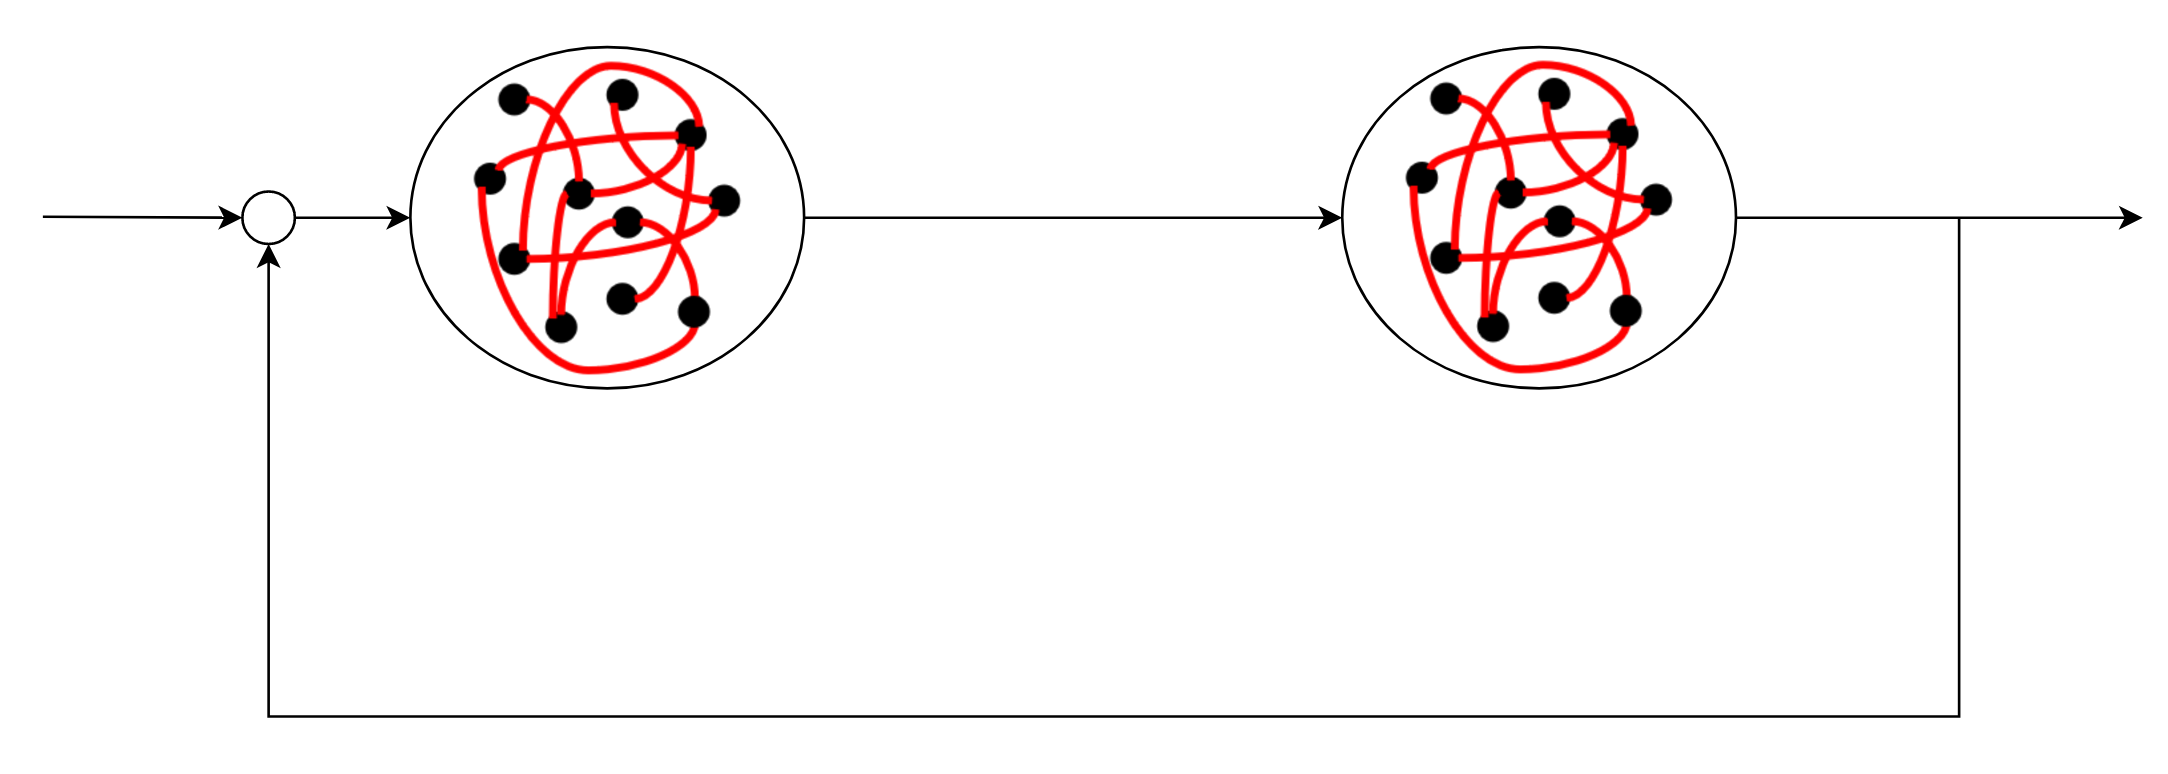
\includegraphics[scale = 0.15]{figures/control_3.png}
				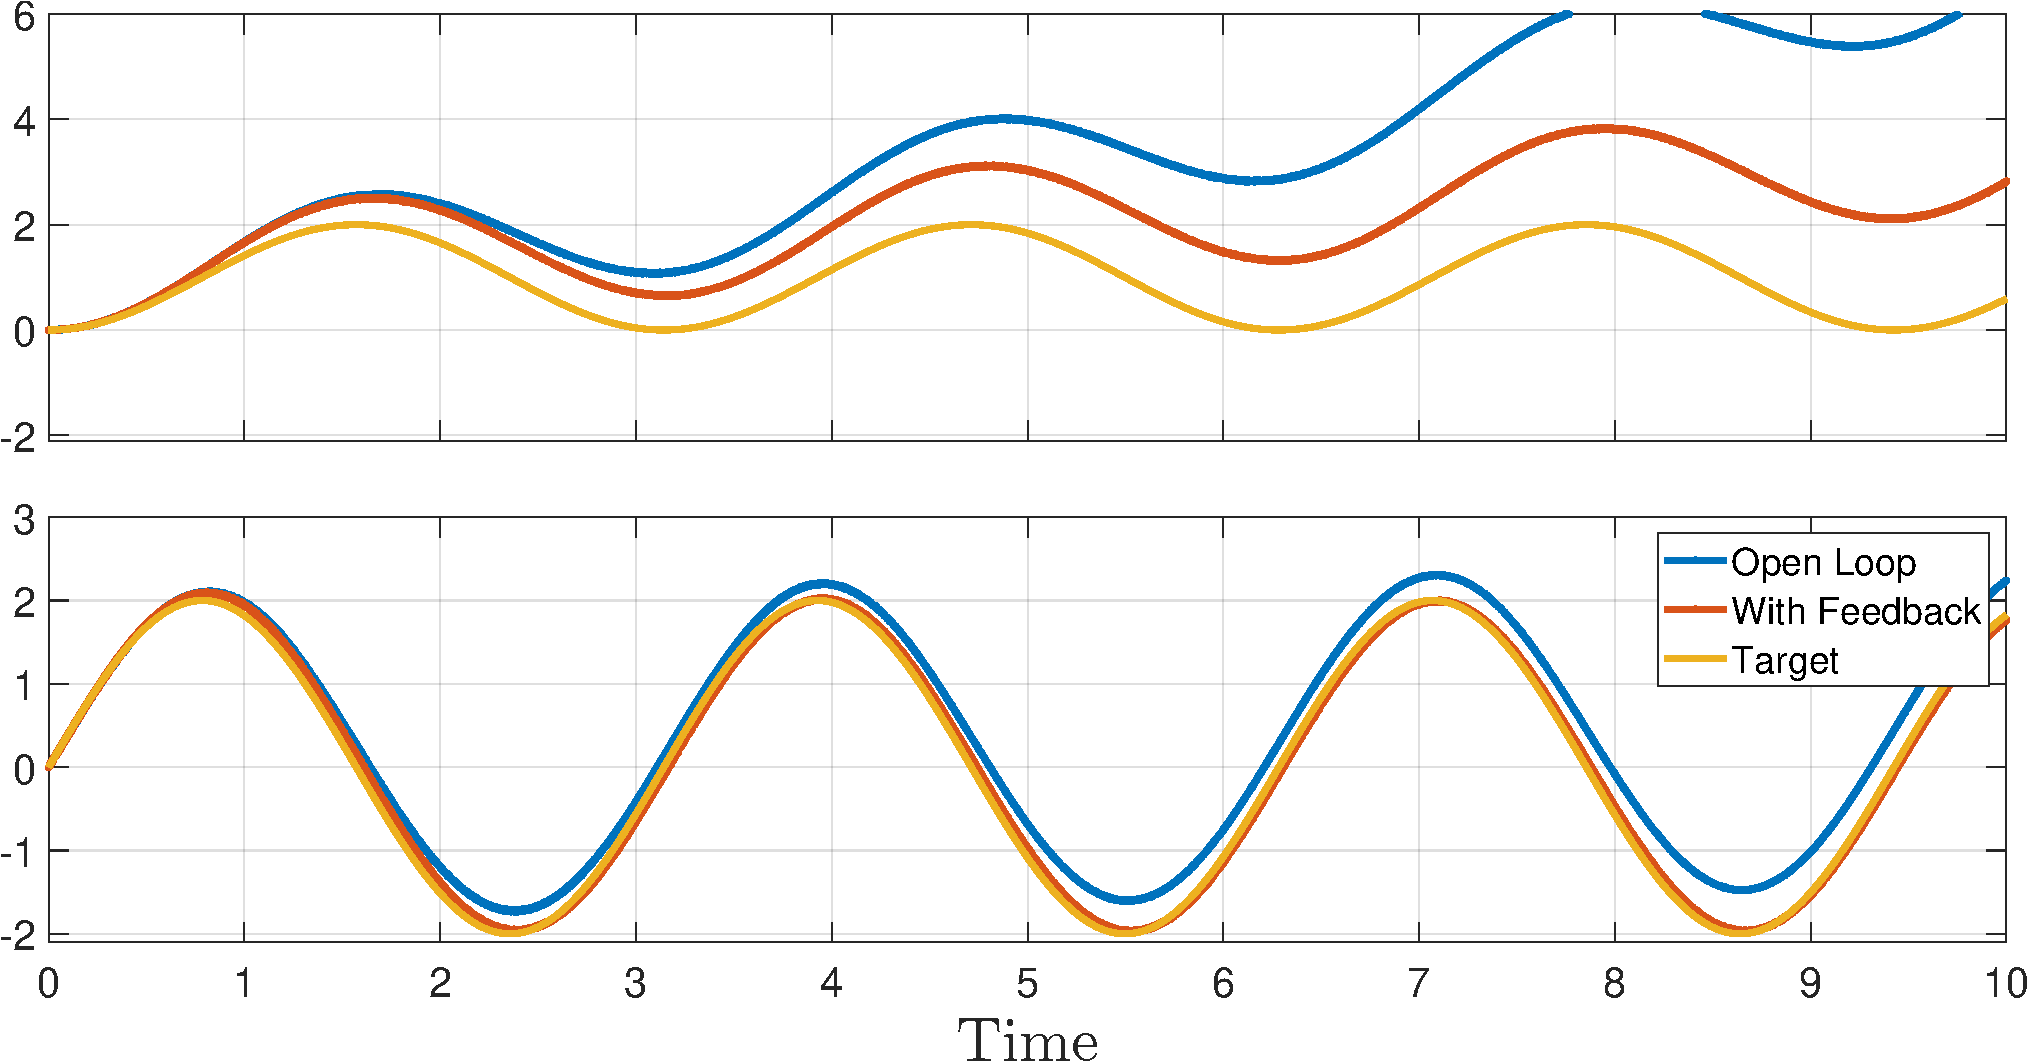
\includegraphics[width = 0.9\textwidth]{figures/plots/everything/feedback_2_nets.pdf}
			\end{figure}
		\end{column}
		\begin{column}{0.45\textwidth}
			% This is 1 single network with Feedback
			\begin{figure}
				\centering
				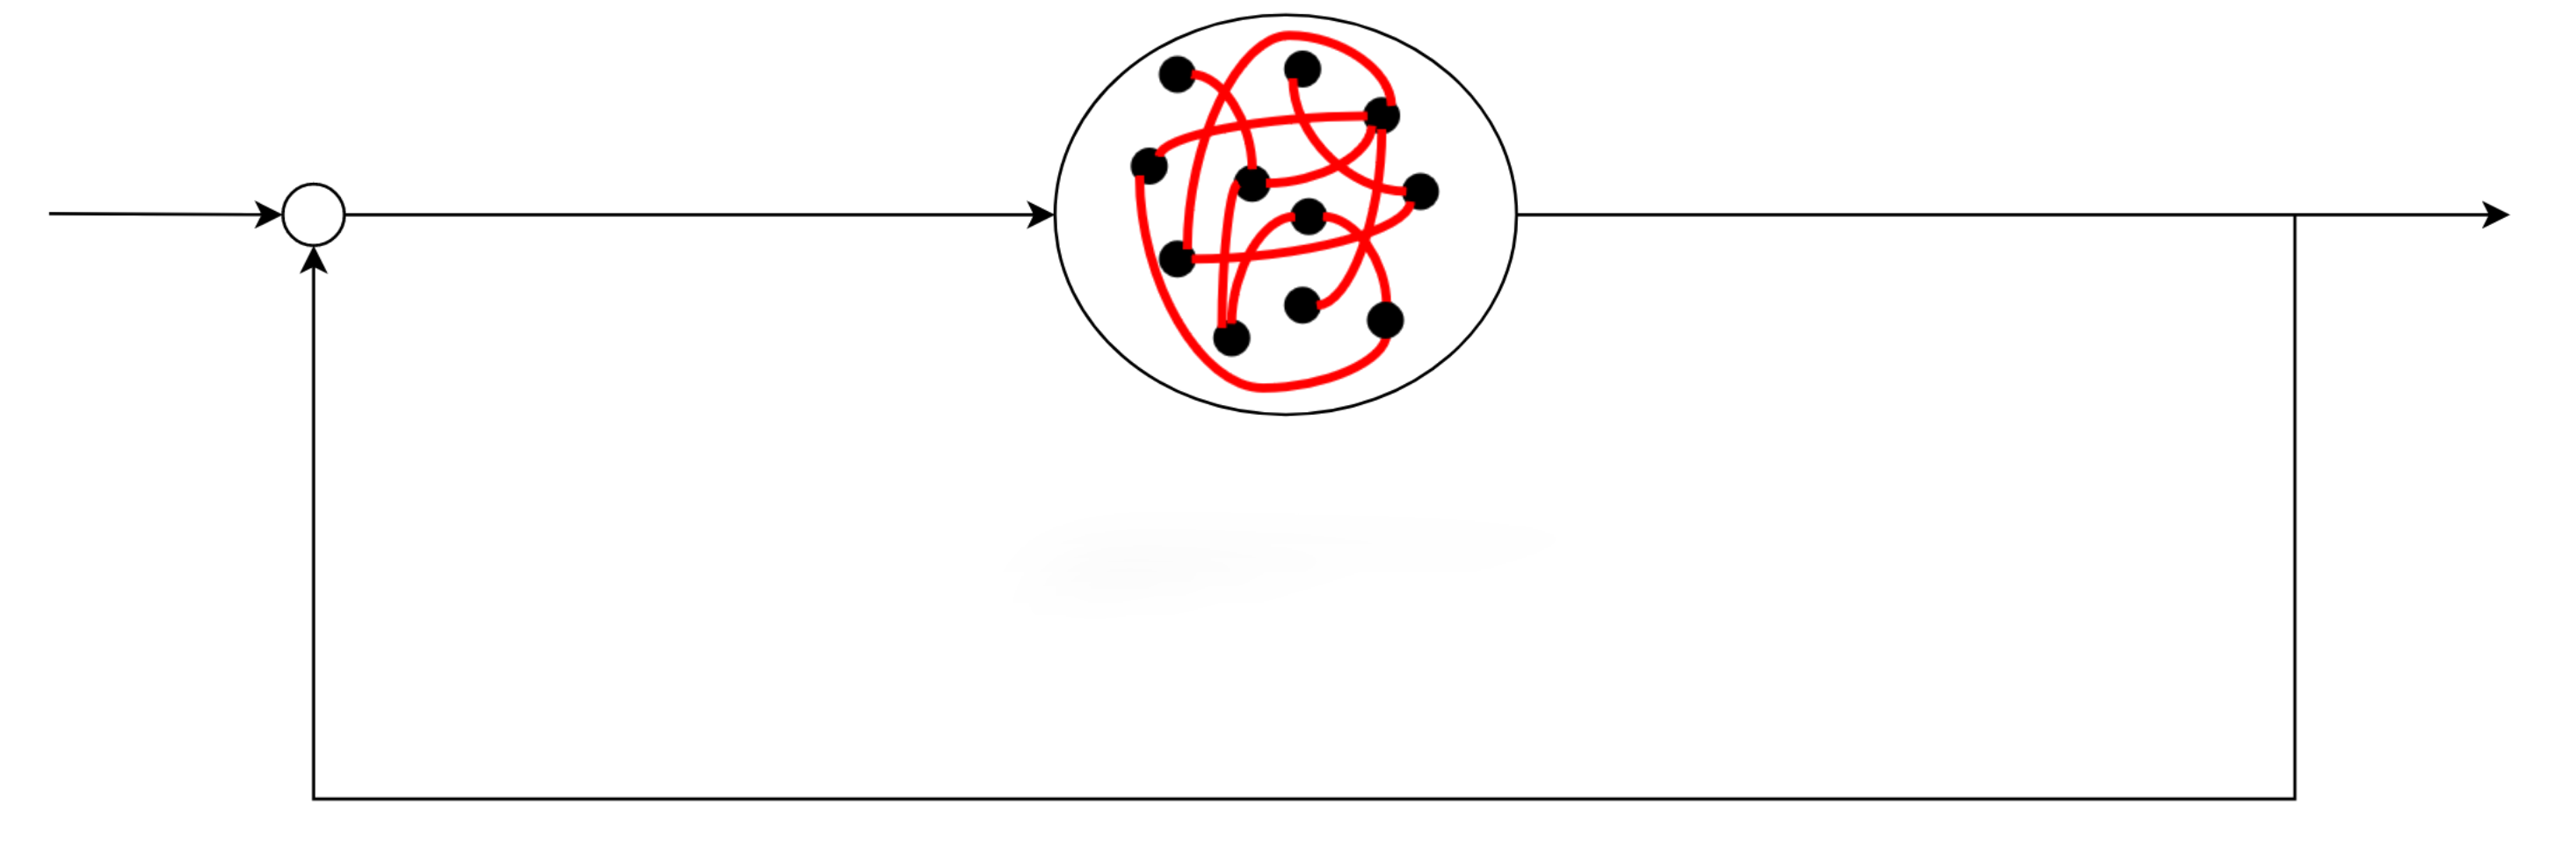
\includegraphics[scale = 0.12]{figures/control_4.png}
				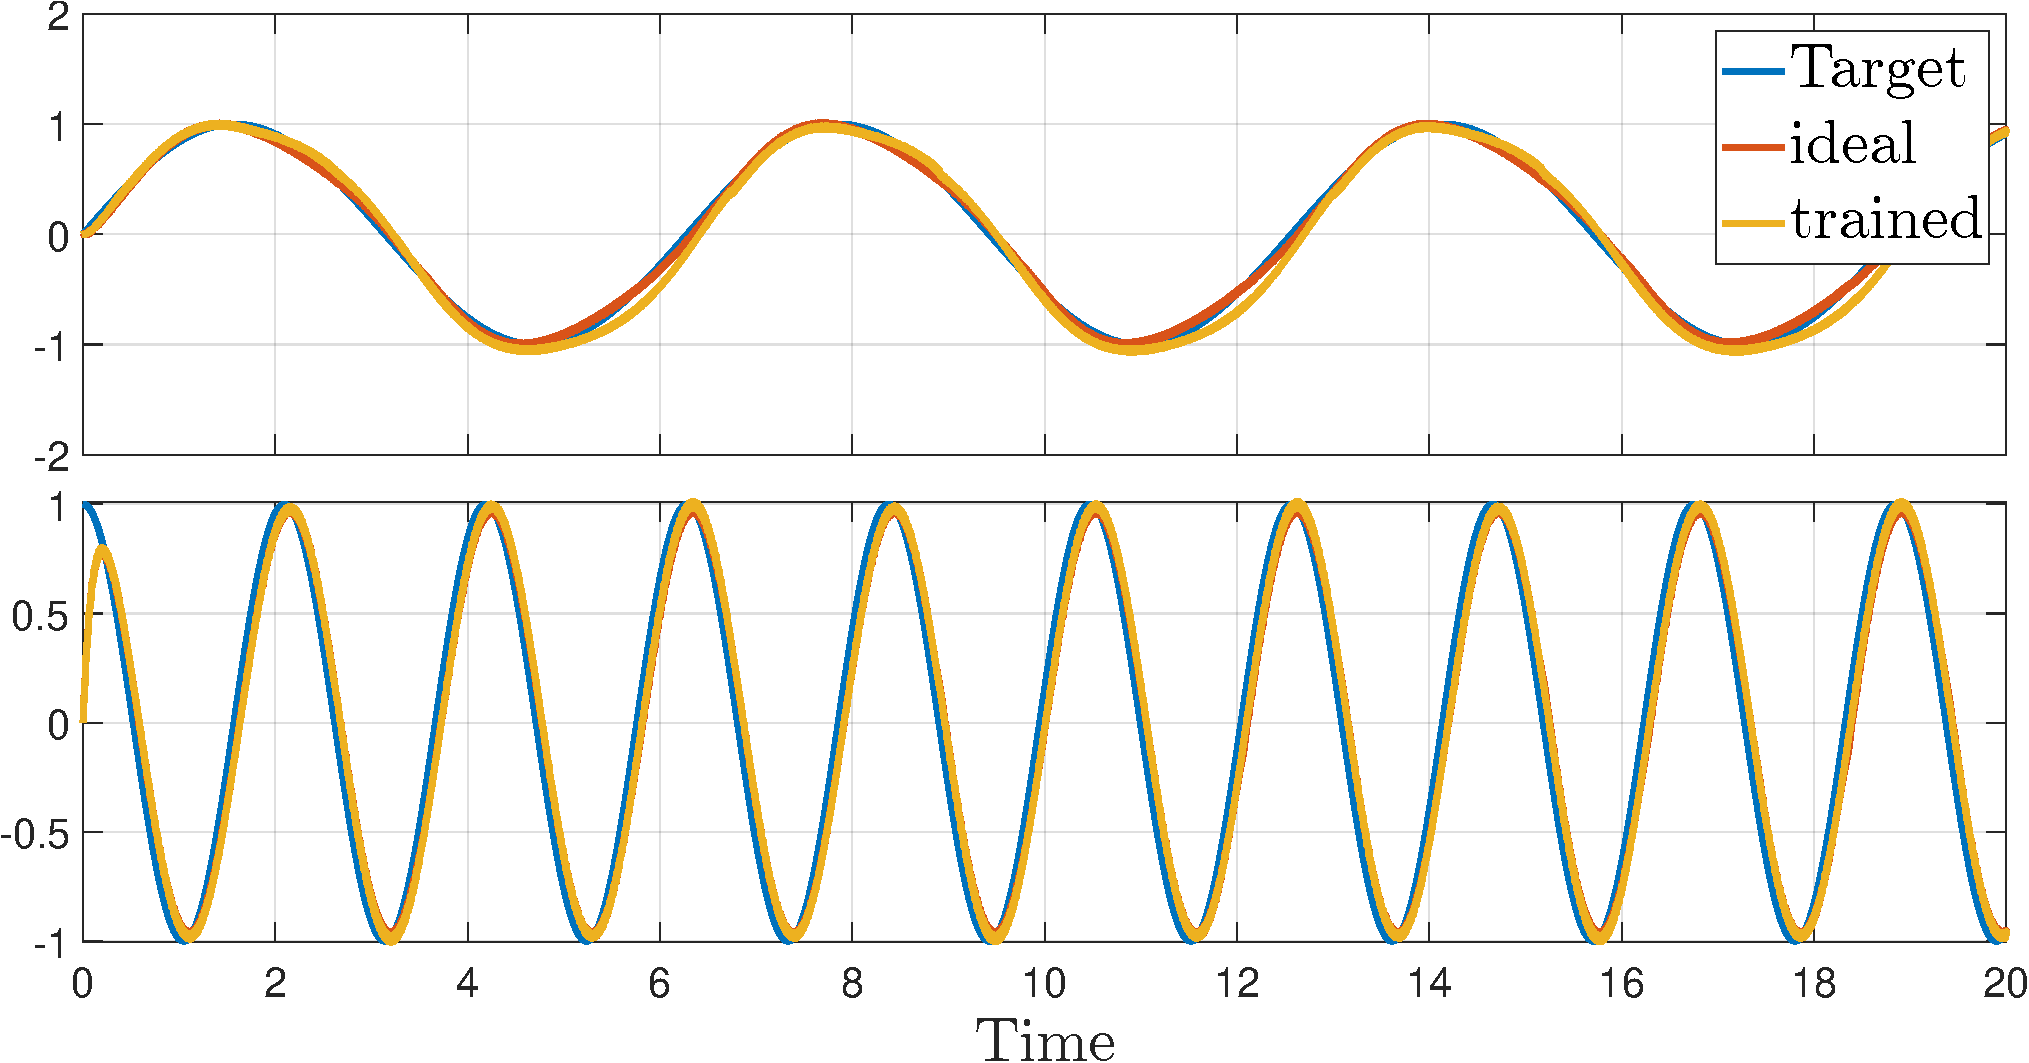
\includegraphics[width = 0.9\textwidth]{figures/plots/everything/all_closed_sine_base.pdf}
			\end{figure}
		\end{column}
	\end{columns}
\end{frame}



\section{Conclusion}\insertsectionpage
\begin{frame}{Conclusion}
	\vspace{-1cm}
	\begin{columns}
		\begin{column}{0.45\textwidth}
			\begin{itemize}
				\setlength\itemsep{0.7em}
				\item Open loop and inaccurate learning of slow weights $W^s$ need to be addressed.
				\item Highly dependent on initial conditions in learning
				\item Impressive accuracy
			\end{itemize}
		\end{column}
		\vrule
		\begin{column}{0.45\textwidth}
			\begin{itemize}
				\setlength\itemsep{0.7em}
				\item In ideal conditions useable results achievable
				\item Limited Applicability $\rightarrow$ Only of theoretical Interest
				\item Results are somewhat translatable to NEF and LSMs
			\end{itemize}
		\end{column}
	\end{columns}
	\vspace{0.5cm}
	Choice between biologic plausibility or and Input Matrix Restriction for accurate results
\end{frame}







\begin{frame}{Future Work}
	\begin{itemize}
		\setlength\itemsep{1.5em}
		\item Enable non-linear dynamics
		\item Obey Dale's Law for neuron excitation and inhibition
		\item Learning of En- and Decoder $F$
		\item Allow for synaptic delays
	\end{itemize}
\end{frame}


\AtNextBibliography{\small}
\begin{frame}[allowframebreaks]{Bibliography}
	\printbibliography
\end{frame}


%\insertendpage







%██████   █████   ██████ ██   ██ ██    ██ ██████      ███████ ██      ██ ██████  ███████ ███████
%██   ██ ██   ██ ██      ██  ██  ██    ██ ██   ██     ██      ██      ██ ██   ██ ██      ██
%██████  ███████ ██      █████   ██    ██ ██████      ███████ ██      ██ ██   ██ █████   ███████
%██   ██ ██   ██ ██      ██  ██  ██    ██ ██               ██ ██      ██ ██   ██ ██           ██
%██████  ██   ██  ██████ ██   ██  ██████  ██          ███████ ███████ ██ ██████  ███████ ███████


\section*{BackupSlides}\insertsectionpage




\begin{frame}{Takeaways}
	\begin{alertblock}{Do not trust the plots}
		\begin{columns}
			\begin{column}{0.48\textwidth}
				\begin{figure}
					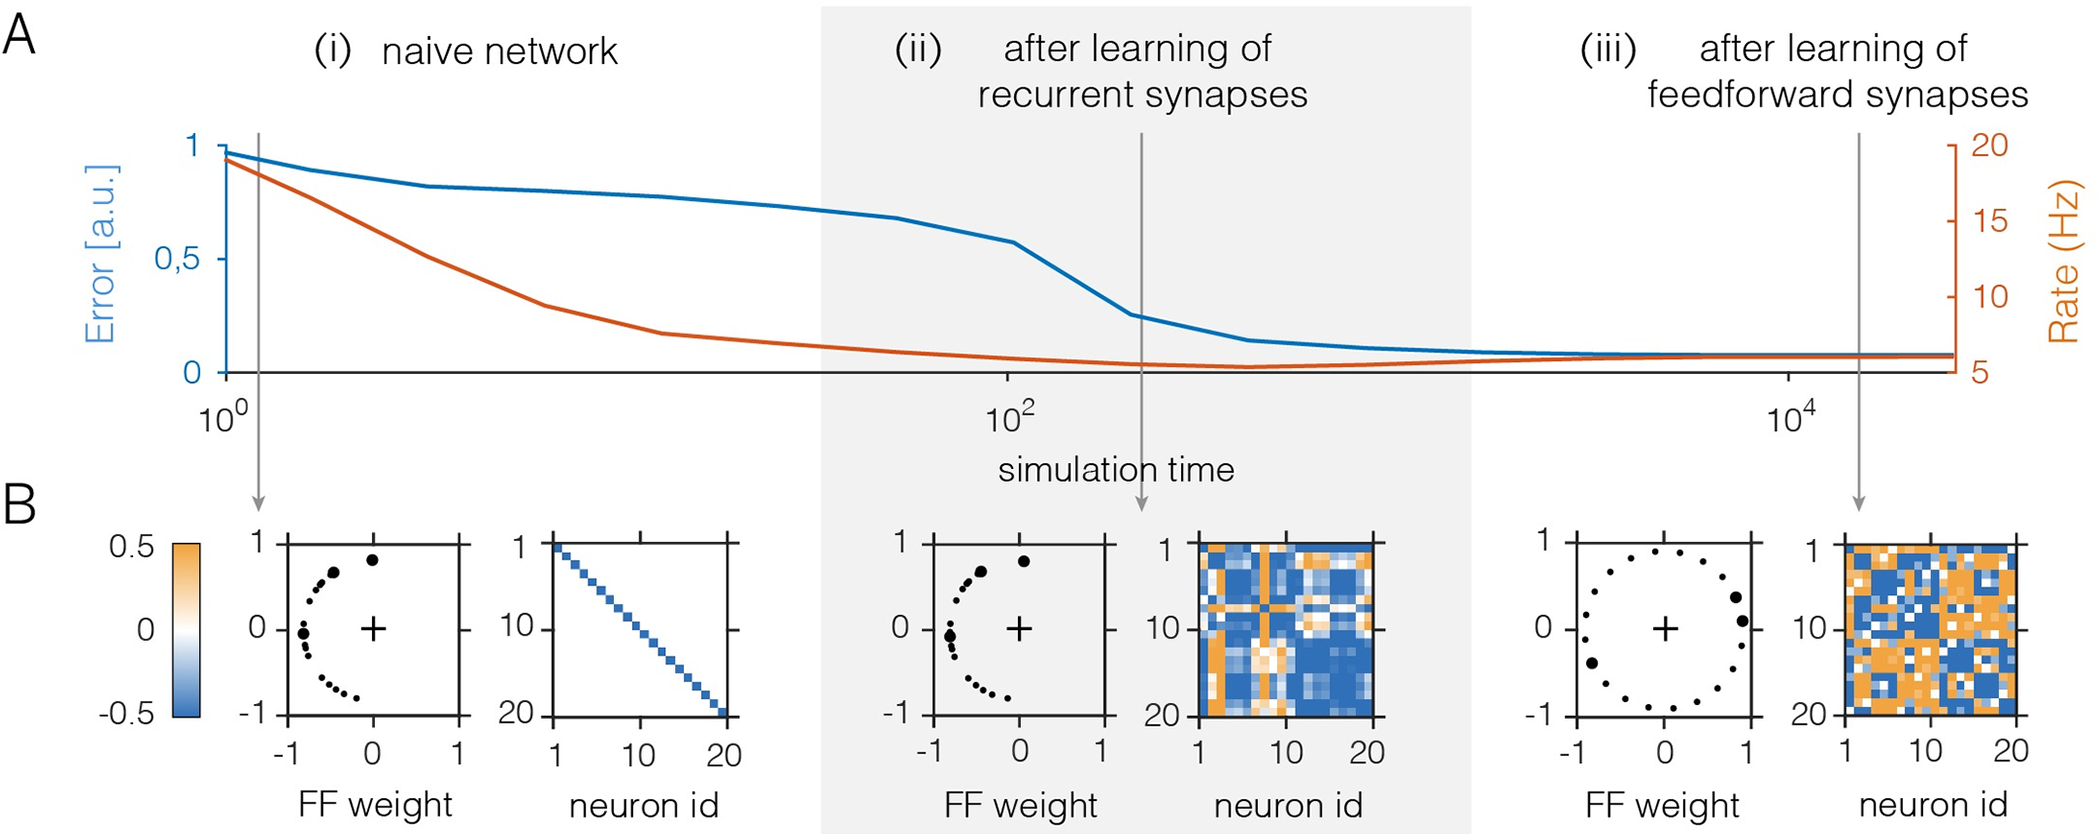
\includegraphics[width= 0.8\textwidth]{figures/fake1.png}
				\end{figure}
			Not the learned decoder! \cite{brendel_learning_2020}
			\end{column}

		\begin{column}{0.48\textwidth}
			\begin{figure}
				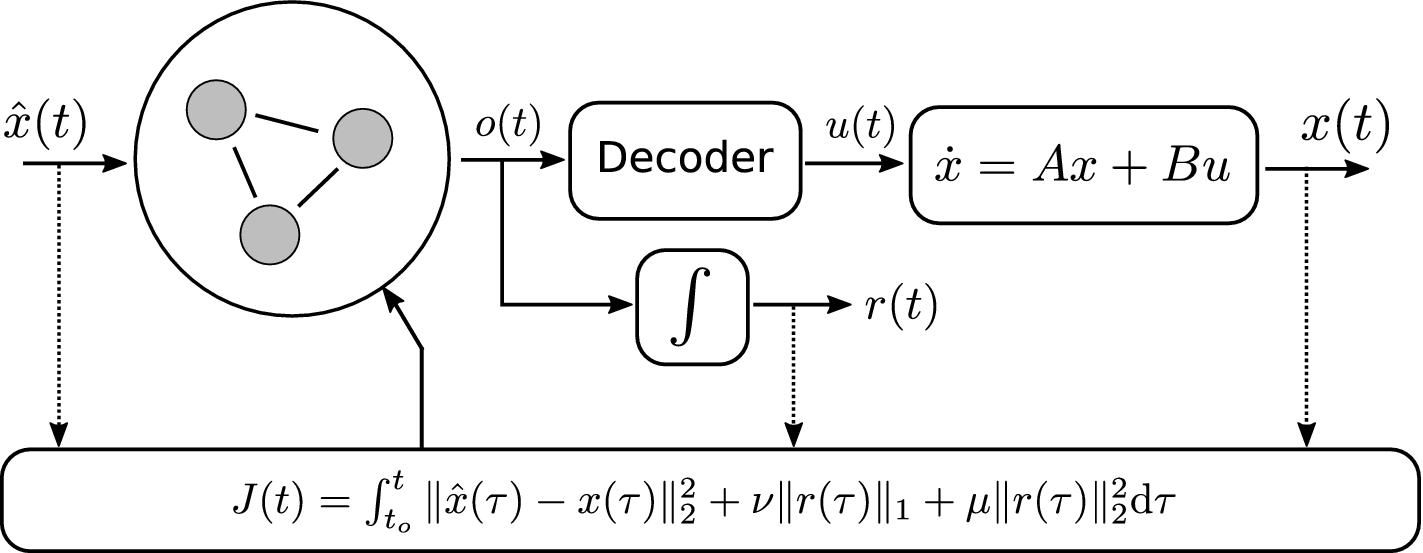
\includegraphics[width= 0.8\textwidth]{figures/fake2.png}
			\end{figure}
			No Control Loop! \cite{huang_spiking_2019}
		\end{column}
		\end{columns}
	\end{alertblock}
\end{frame}



\begin{frame}{Autoencoder}
	\begin{columns}[T]
		\begin{column}{0.48\textwidth}
			\begin{center}
				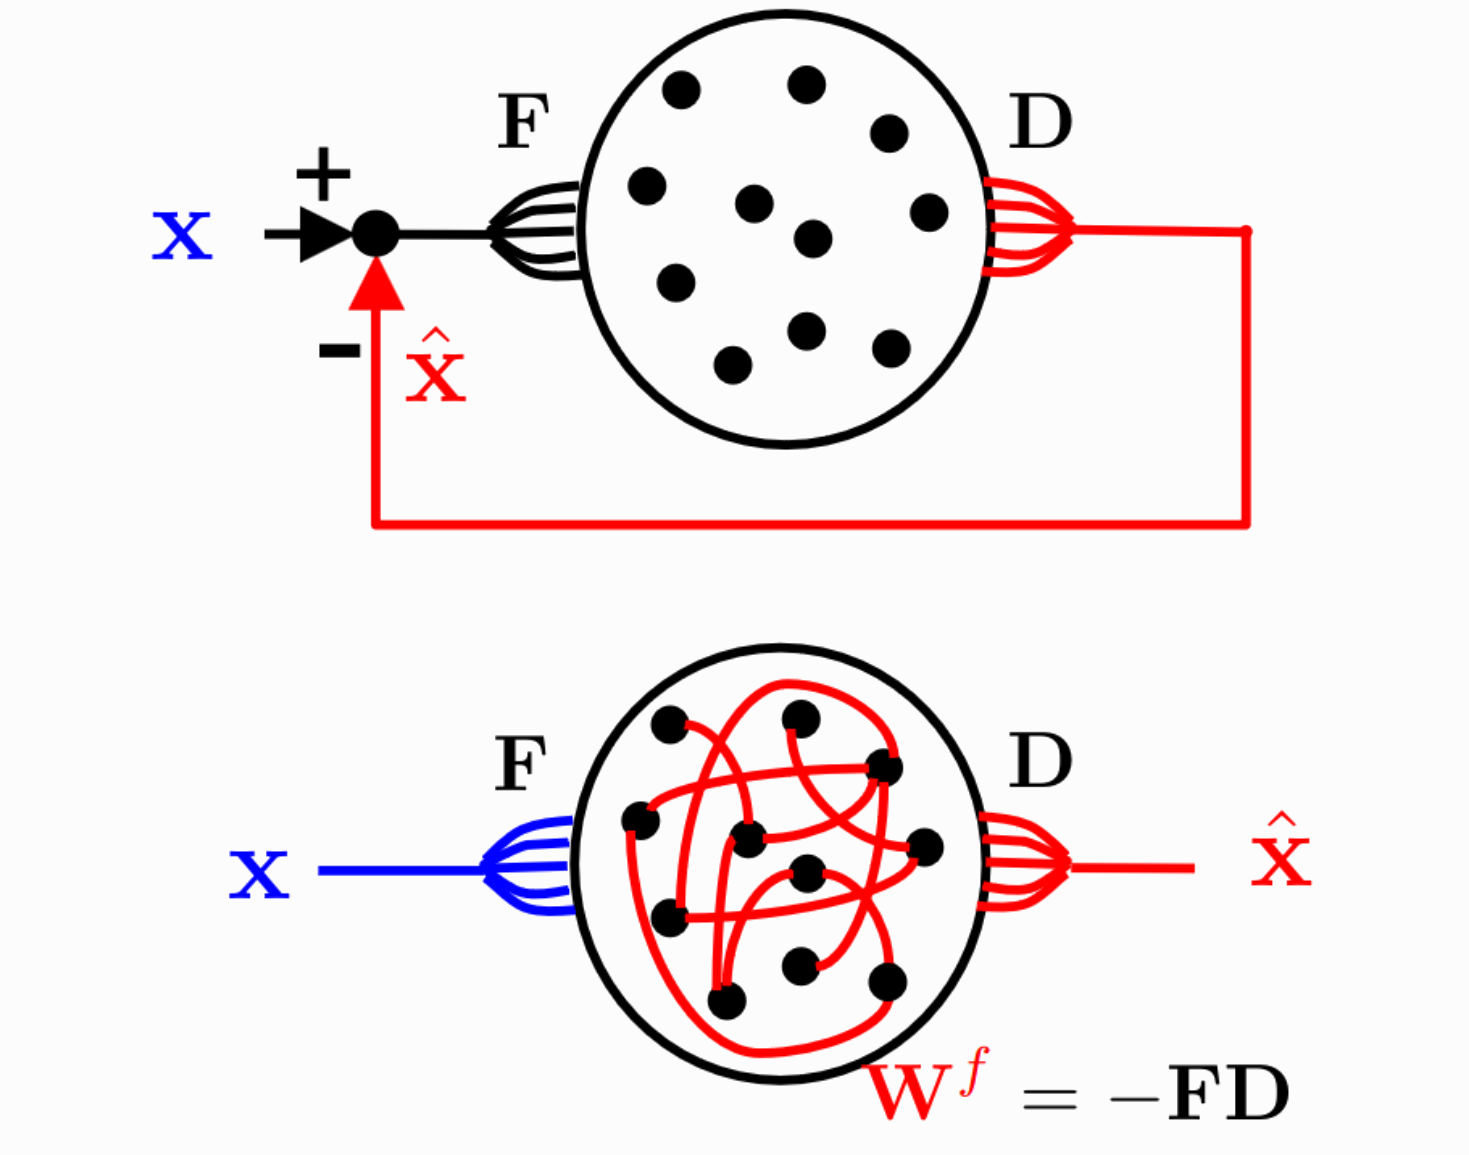
\includegraphics[width=0.9\textwidth,trim= 3cm 5cm 3cm 6cm]{figures/autoencoder.png}
			\end{center}
		\end{column}

		\begin{column}{0.48\textwidth}
			\begin{center}
				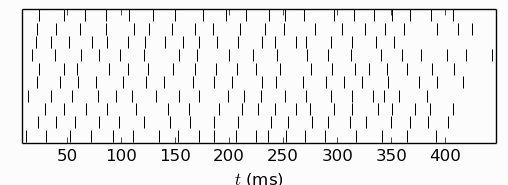
\includegraphics[width=0.9\textwidth]{figures/spikeplot.png}
			\end{center}
			\begin{equation}
				\begin{aligned}
					\hat{x} &= Do(t)\\
					\dot{r} &= -\lambda r + o(t)
				\end{aligned}
			\end{equation}
		\end{column}
	\end{columns}

\end{frame}


\begin{frame}{Autoencoder II}
	\begin{textblock*}{10pt}(550pt,20pt)
		\small
		\begin{equation*}
		\dot{r} = -\lambda r + \sigma(t)
		\end{equation*}
	\end{textblock*}
	\begin{columns}[T]
		\begin{column}{0.48\textwidth}
			\begin{center}
				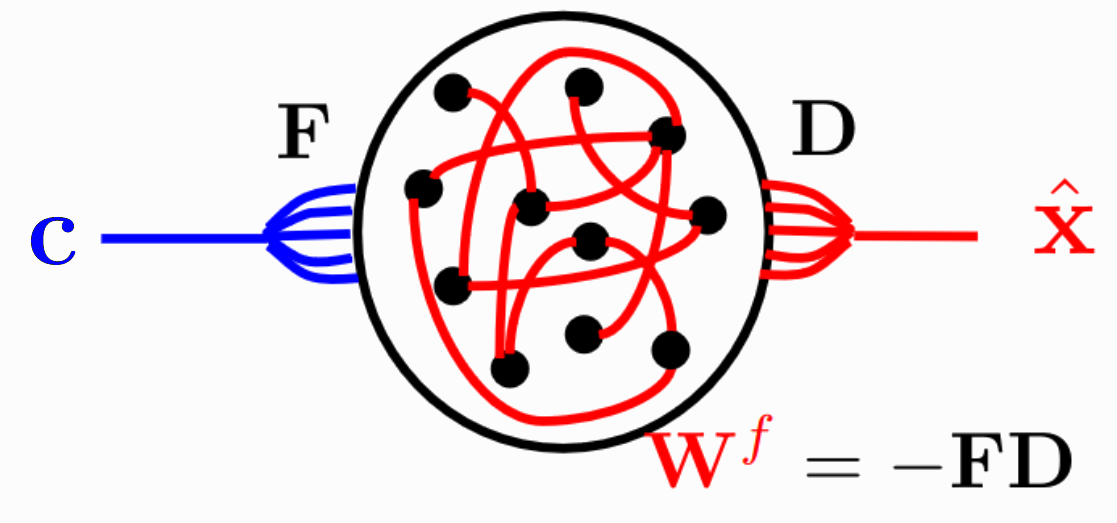
\includegraphics[width=0.9\textwidth,trim= 3cm 5cm 3cm 0cm]{figures/autoencoder2.png}
			\end{center}
		\end{column}

		\begin{column}{0.48\textwidth}
			\begin{equation}
			\begin{aligned}
			\dot{x} &= -\lambda x + c\\
			\hat{x} &= Dr
			\end{aligned}
			\end{equation}
		\end{column}
	\end{columns}

\end{frame}


\begin{frame}{Autoencoder III}
	\begin{textblock*}{10pt}(550pt,20pt)
		\small
		\begin{equation*}
			\begin{aligned}
				\dot{r} &= -\lambda r + o(t)\\
				\hat{x} &= Dr
			\end{aligned}
		\end{equation*}
	\end{textblock*}
	\begin{columns}[T]
		\begin{column}{0.48\textwidth}
			\begin{center}
				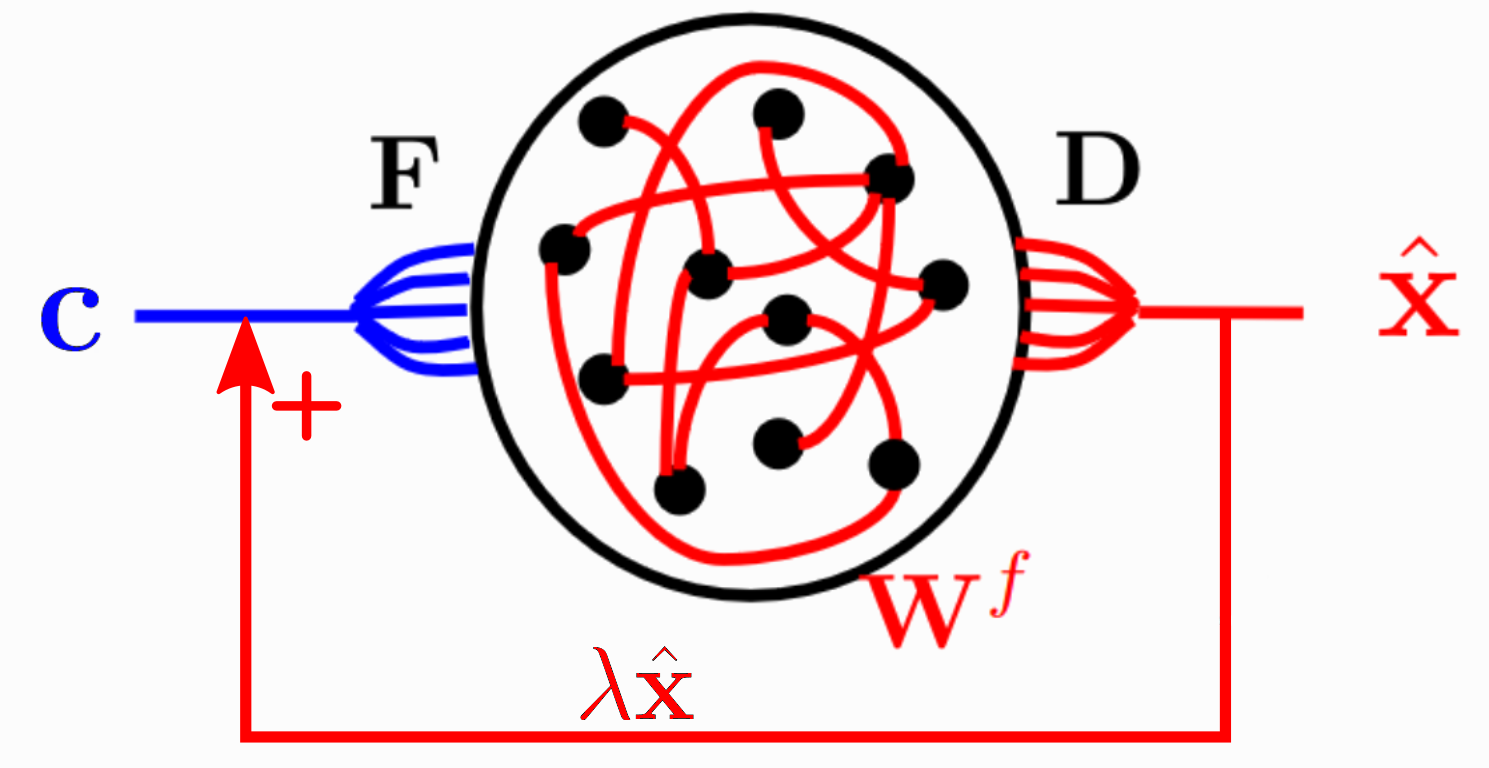
\includegraphics[width=0.9\textwidth,trim= 3cm 3cm 3cm 0cm]{figures/autoencoder3.png}
			\end{center}

			\begin{equation}
			\dot{x} = c
			\end{equation}
		\end{column}

		\begin{column}{0.48\textwidth}
			\begin{center}
				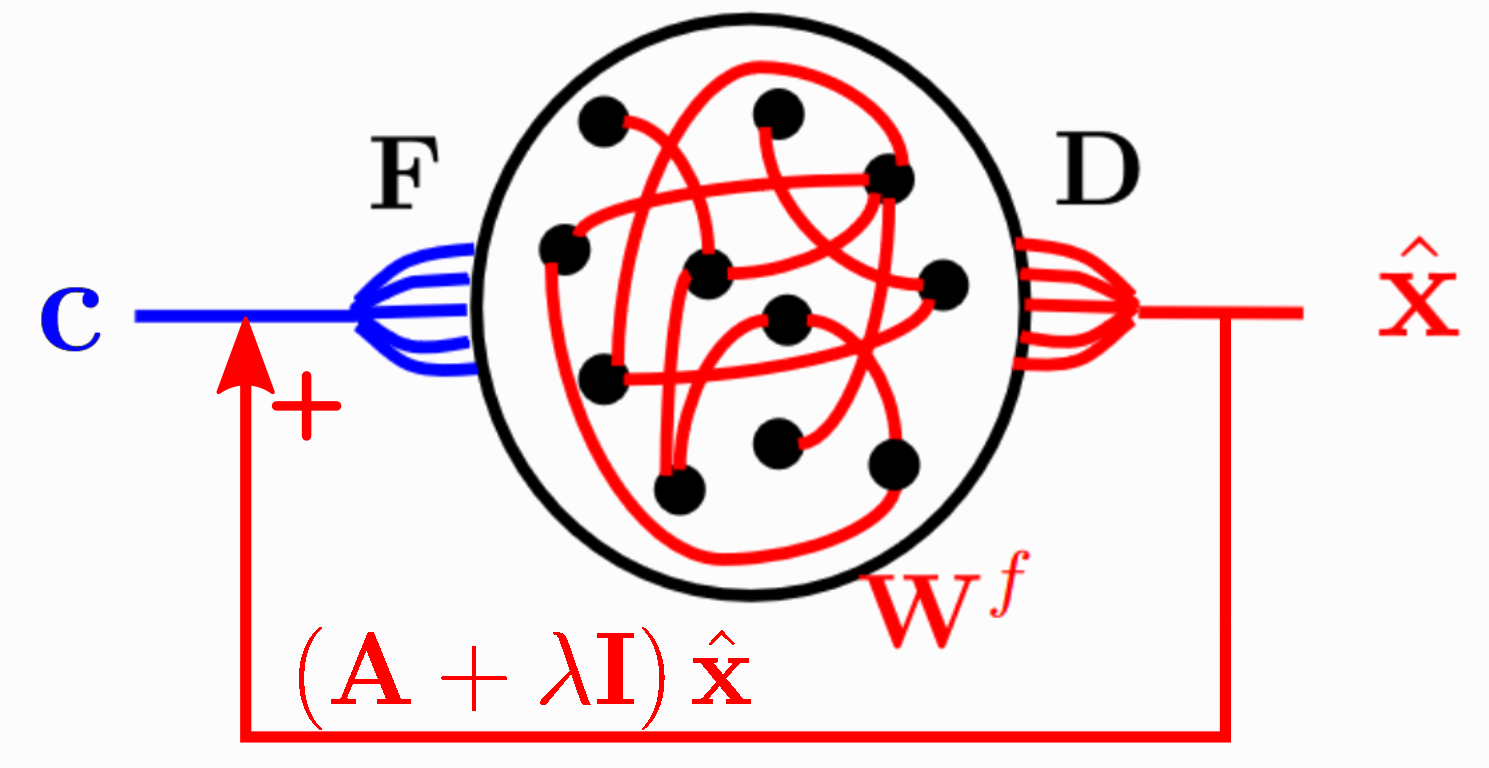
\includegraphics[width=0.9\textwidth,trim= 3cm 3cm 3cm 0cm]{figures/autoencoder4.png}
			\end{center}

			\begin{equation}
			\dot{x} = Ax + c
			\end{equation}
		\end{column}
	\end{columns}
\end{frame}

\begin{frame}{Geometric}
	\only<1->{
	\begin{tikzpicture}[remember picture, overlay]
		\node at (current page.north east) [xshift=-20cm, yshift=-8.85cm] {
		\begin{tikzpicture}
		\begin{axis}[
		width=0.35\textwidth,
		height=0.35\textwidth,
		xlabel={$\Delta x_1$},
		ylabel={$\Delta x_2$},
		xmin =-0.9,
		xmax = 0.9,
		ymin = -0.9,
		ymax = 0.9,
		axis equal,
		axis lines=middle,
		enlargelimits=true,
		xticklabels ={},
		yticklabels = {},
		xlabel style={
			at={(ticklabel* cs:1.02)}, % Adjust the position of xlabel
			anchor=north,
		},
		ylabel style={
			at={(ticklabel* cs:1.02)}, % Adjust the position of ylabel
			anchor=south,
		},
		]
		\draw[->,violet,ultra thick](axis cs:0,0.0)--(axis cs: 0.5,0.5) node[midway,left,text=violet]{$\color{violet} F_1$};
		\draw[->,teal,ultra thick](axis cs:0,0.0)--(axis cs: -0.5,0.5)node[midway,left,text=violet]{$\color{teal} F_2$};
		\draw[->,red,ultra thick](axis cs:0,0.0)--(axis cs: 0.5,-0.5)node[midway,right,text=violet]{$\color{red} F_4$};
		\draw[->,orange,ultra thick](axis cs:0,0.0)--(axis cs: -0.5,-0.5)node[midway,left,text=violet]{$\color{orange} F_3$};
		\draw[draw = none,top color = white, middle color = white,bottom color = violet,shading angle = -90,opacity = 0.6,transform canvas = {rotate around={45:(axis cs: 0.0,0.0)}}] (axis cs:0.707,-5) rectangle (axis cs:0.9,5);
		\draw[draw = none,top color = white, middle color = white,bottom color = teal,shading angle = -90,opacity = 0.6,transform canvas = {rotate around={135:(axis cs: 0.0,0.0)}}] (axis cs:0.707,-5) rectangle (axis cs:0.9,5);
		\draw[draw = none,top color = white, middle color = white,bottom color = orange,shading angle = -90,opacity = 0.6,transform canvas = {rotate around={225:(axis cs: 0.0,0.0)}}] (axis cs:0.707,-5) rectangle (axis cs:0.9,5);
		\draw[draw = none,top color = white, middle color = white,bottom color = red,shading angle = -90,opacity = 0.6,transform canvas = {rotate around={-45:(axis cs: 0.0,0.0)}}] (axis cs:0.707,-5) rectangle (axis cs:0.9,5);

		\end{axis}
		\end{tikzpicture}};
	\end{tikzpicture}
	}

	\only<1>{
	\begin{tikzpicture}[remember picture, overlay]
		\node at (current page.north east) [xshift=-8cm, yshift=-7.5cm] {
		\begin{tikzpicture}
		\begin{axis}[
		width=0.5\textwidth,
		height=0.3\textwidth,
		xlabel={$x_1$},
		ylabel={$x_2$},
		domain=0:3.5,
		samples=100,
		axis lines=middle,
		enlargelimits=true,
		clip mode=individual, % Ensure everything is shown
		xticklabels ={},
		yticklabels = {},
		xlabel style={
		at={(ticklabel* cs:0.5)}, % Adjust the position of xlabel
			anchor=north,
		},
		ylabel style={
			at={(ticklabel* cs:0.5)}, % Adjust the position of ylabel
			anchor=south,
			rotate=90, % Rotate ylabel by 90 degrees
		},
		]
		\addplot[blue,thick] {0.28934*x^3 - 1.8178*x^2 + 2.6016*x^1 + 0.66431};
		\draw[->,violet,ultra thick](axis cs:0,0.66)--(axis cs: 0.353553,1.01355);
		\draw[->,teal,ultra thick](axis cs:0.353553,1.01355)--(axis cs: 5.55112e-17,1.36711);
		\draw[->,violet,ultra thick](axis cs:5.55112e-17,1.36711)--(axis cs: 0.353553,1.72066);
		\draw[->,red,ultra thick](axis cs:0.353553,1.72066)--(axis cs: 0.707107,1.36711);
		\draw[->,violet,ultra thick](axis cs:0.707107,1.36711)--(axis cs: 1.06066,1.72066);
		\draw[->,red,ultra thick](axis cs:1.06066,1.72066)--(axis cs: 1.41421,1.36711);
		\draw[->,red,ultra thick](axis cs:1.41421,1.36711)--(axis cs: 1.76777,1.01355);
		\draw[->,red,ultra thick](axis cs:1.76777,1.01355)--(axis cs: 2.12132,0.66);
		\draw[->,red,ultra thick](axis cs:2.12132,0.66)--(axis cs: 2.47487,0.306447);
		\draw[->,red,ultra thick](axis cs:2.47487,0.306447)--(axis cs: 2.82843,-0.0471068);
		\draw[->,red,ultra thick](axis cs:2.82843,-0.0471068)--(axis cs: 3.18198,-0.40066);
		\draw[->,violet,ultra thick](axis cs:3.18198,-0.40066)--(axis cs: 3.53553,-0.0471068);
		\end{axis}
		\end{tikzpicture}};
	\end{tikzpicture}
	}

	\only<2->{
	\begin{columns}[T]
		\begin{column}{0.2\textwidth}

		\end{column}
		\begin{column}{0.6\textwidth}
			Minimize the cost $J$ (Greedy)\\
			\begin{equation}
				J = \int_{0}^{T} \|x-\hat{x}\|^2_2 + C(r) \ dt
			\end{equation}
			\begin{equation}
			\begin{aligned}
				V_i=&F_i(x-\hat{x}) - \mu r_i\\
				\dot{V}_i=&-\lambda_V V_i+F_ic(t)\\
				&+ W^fo(t) + W^sr(t)+\sigma_V \eta(t)\\
				W^f =& FF^T+ \mu I\\
				W^s =& F\left(A + \lambda_dI\right)F^T
			\end{aligned}
			\end{equation}
		\end{column}
	\end{columns}
	}

\end{frame}


%\section{Control}\insertsectionpage

\begin{frame}{Control Concept}
	\begin{center}
		\begin{tikzpicture}
		% Include the picture
			\node[anchor=south west, inner sep=0] (image) at (100pt,100pt) {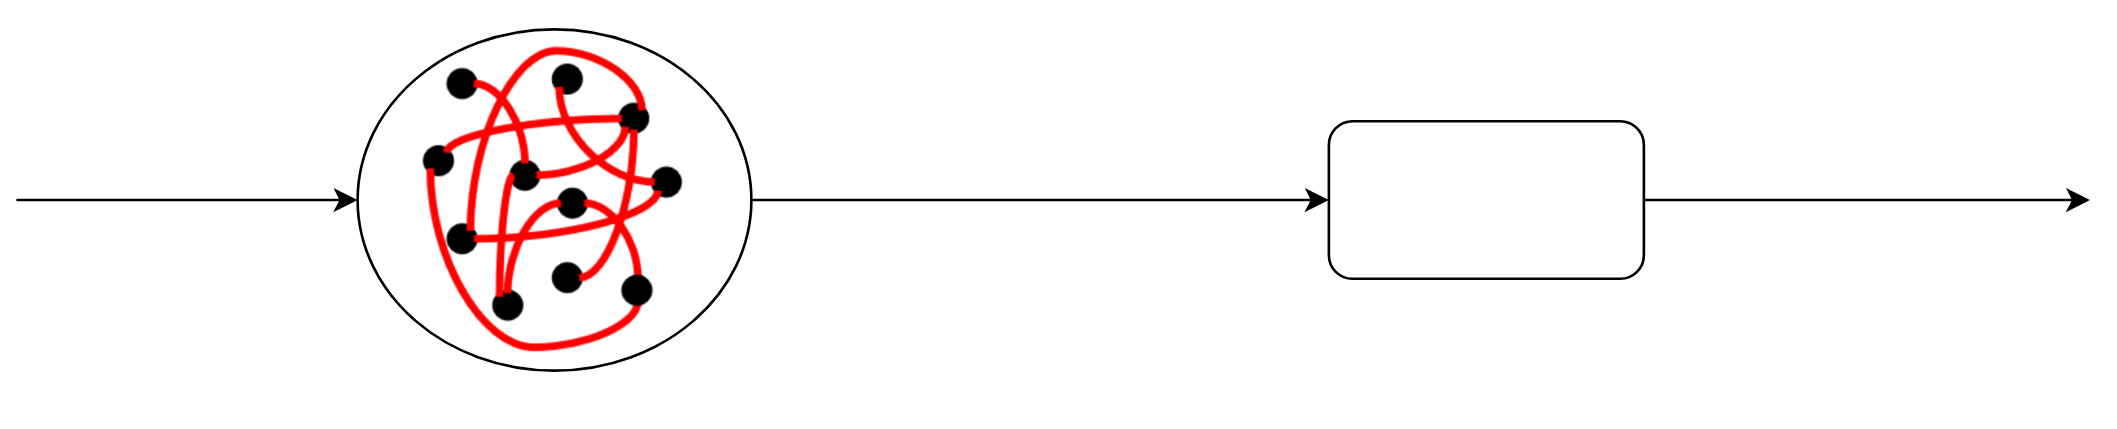
\includegraphics[width=0.7\textwidth]{figures/control_1.png}};

		% Overlay equation
			\node[anchor=south west, align=left, opacity=1] at ([shift={(288pt,25pt)}]image.south west)  {\scalebox{0.7}{$
			\begin{aligned}
			\dot{x} &= Ax + Bu\\
			y &= Cx
			\end{aligned}
			$}};

			\node[anchor=south west, align=left, opacity=1] at ([shift={(380pt,50pt)}]image.south west)  {\scalebox{0.7}{$\hat{x}$}};
			\node[anchor=south west, align=left, opacity=1] at ([shift={(210pt,50pt)}]image.south west)  {\scalebox{0.7}{$c$}};
			\node[anchor=south west, align=left, opacity=1] at ([shift={(30pt,50pt)}]image.south west)  {\scalebox{0.7}{$\text{x}$}};
		\end{tikzpicture}
		%^^ add some separator here to control the distance between both plots
		\begin{tikzpicture}
		% Include the picture
			\node[anchor=south west, inner sep=0] (image) at (100pt,100pt) {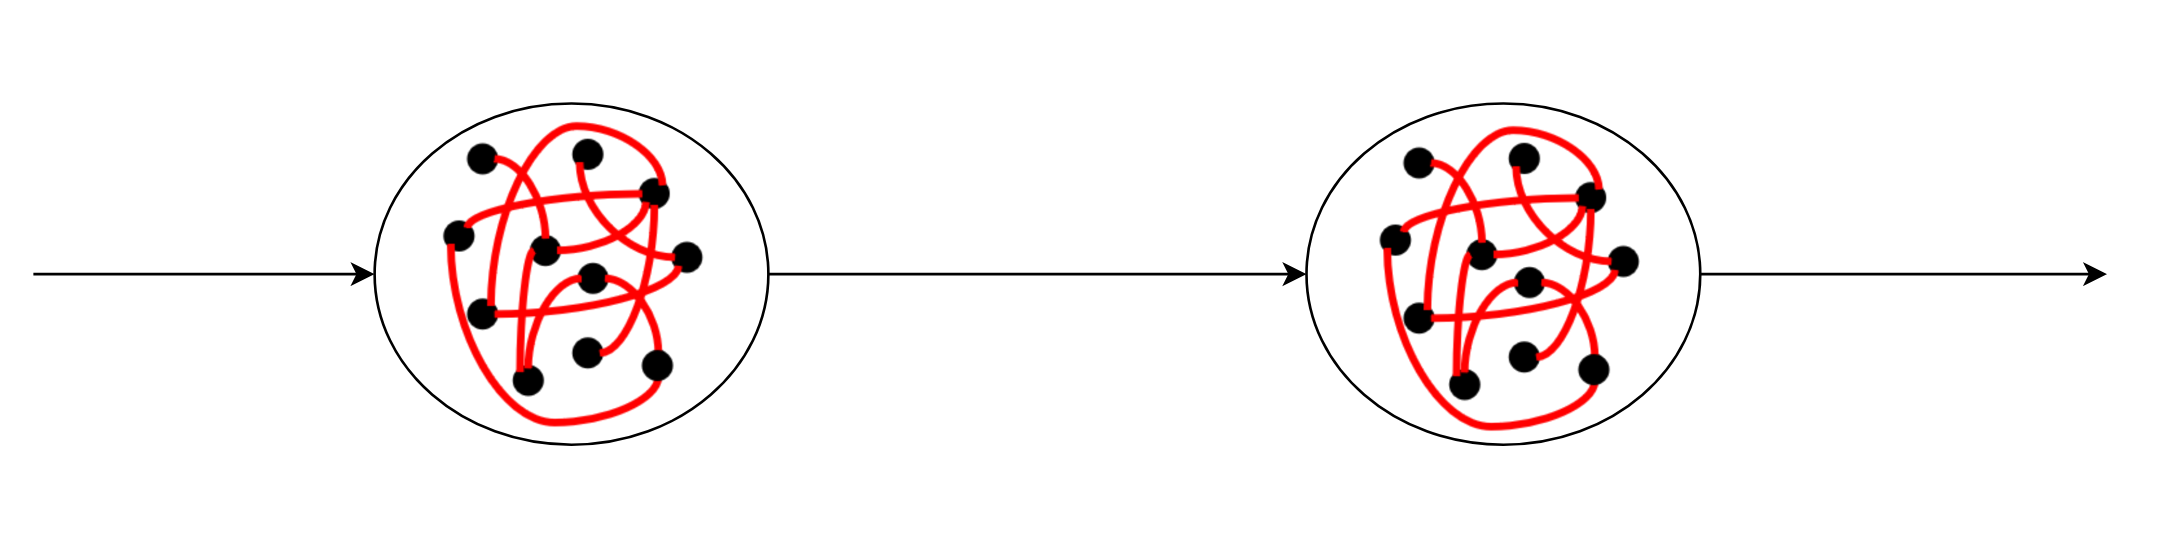
\includegraphics[width=0.7\textwidth]{figures/control_2.png}};

		\node[anchor=south west, align=left, opacity=1] at ([shift={(380pt,60pt)}]image.south west)  {\scalebox{0.7}{$\hat{x}$}};
		\node[anchor=south west, align=left, opacity=1] at ([shift={(210pt,60pt)}]image.south west)  {\scalebox{0.7}{$c$}};
		\node[anchor=south west, align=left, opacity=1] at ([shift={(30pt,60pt)}]image.south west)  {\scalebox{0.7}{$\text{x}$}};
		\end{tikzpicture}

	\end{center}
	\begin{textblock*}{50pt}(650pt,180pt)
		\small
		\cite{huang_spiking_2019}
	\end{textblock*}
\end{frame}

\begin{frame}{Control with SNN}
	\begin{columns}
		\begin{column}{0.45\textwidth}
			\begin{equation}
				u = F^T r + \Omega o(t)
			\end{equation}
			Slow and Instantaneous decoding\\
			\begin{equation}
			\begin{aligned}
			\dot{V}(t)= & -\lambda_V V(t)+\Omega^{\mathrm{T}} B^T A e(t)+\Omega^{\mathrm{T}} B^T c(t) \\
			& +W^s r(t)+W^f o(t)+\sigma_v \eta(t)
			\end{aligned}
			\end{equation}
			Requires full state information on $x$ and $\hat{x}$
			\begin{equation}
				c= \dot{x} - Ax
			\end{equation}
		\end{column}
		\begin{column}{0.45\textwidth}
			It is necessary on $B \in \mathbb{R}^{nxp}$
			\begin{equation}
				\rank(B^TC^T) = p
			\end{equation}
		\end{column}
	\end{columns}
\end{frame}


\begin{frame}{Conclusion}
	\begin{itemize}
		\setlength\itemsep{1.5em}
		\item Acceptable results in ideal conditions

		\item Rank condition is limiting factor

		\item Network noise is invisible to the control

		\item Simple open loop controller in the definition of $c$
	\end{itemize}
\end{frame}

%\section{Learning}\insertsectionpage

\begin{frame}{Slow Learning rule}


	\begin{textblock*}{10pt}(550pt,20pt)
		\small
		\begin{equation*}
		\begin{aligned}
			\dot{\hat{x}}=&(M-K \mathbf{I}) \hat{x}+c+K x\\
			W^s =& F\left(A + \lambda_d\mathbf{I}\right)F^T
		\end{aligned}
		\end{equation*}
	\end{textblock*}

	\begin{columns}
		\begin{column}{0.45\textwidth}
			\begin{figure}
				\centering
				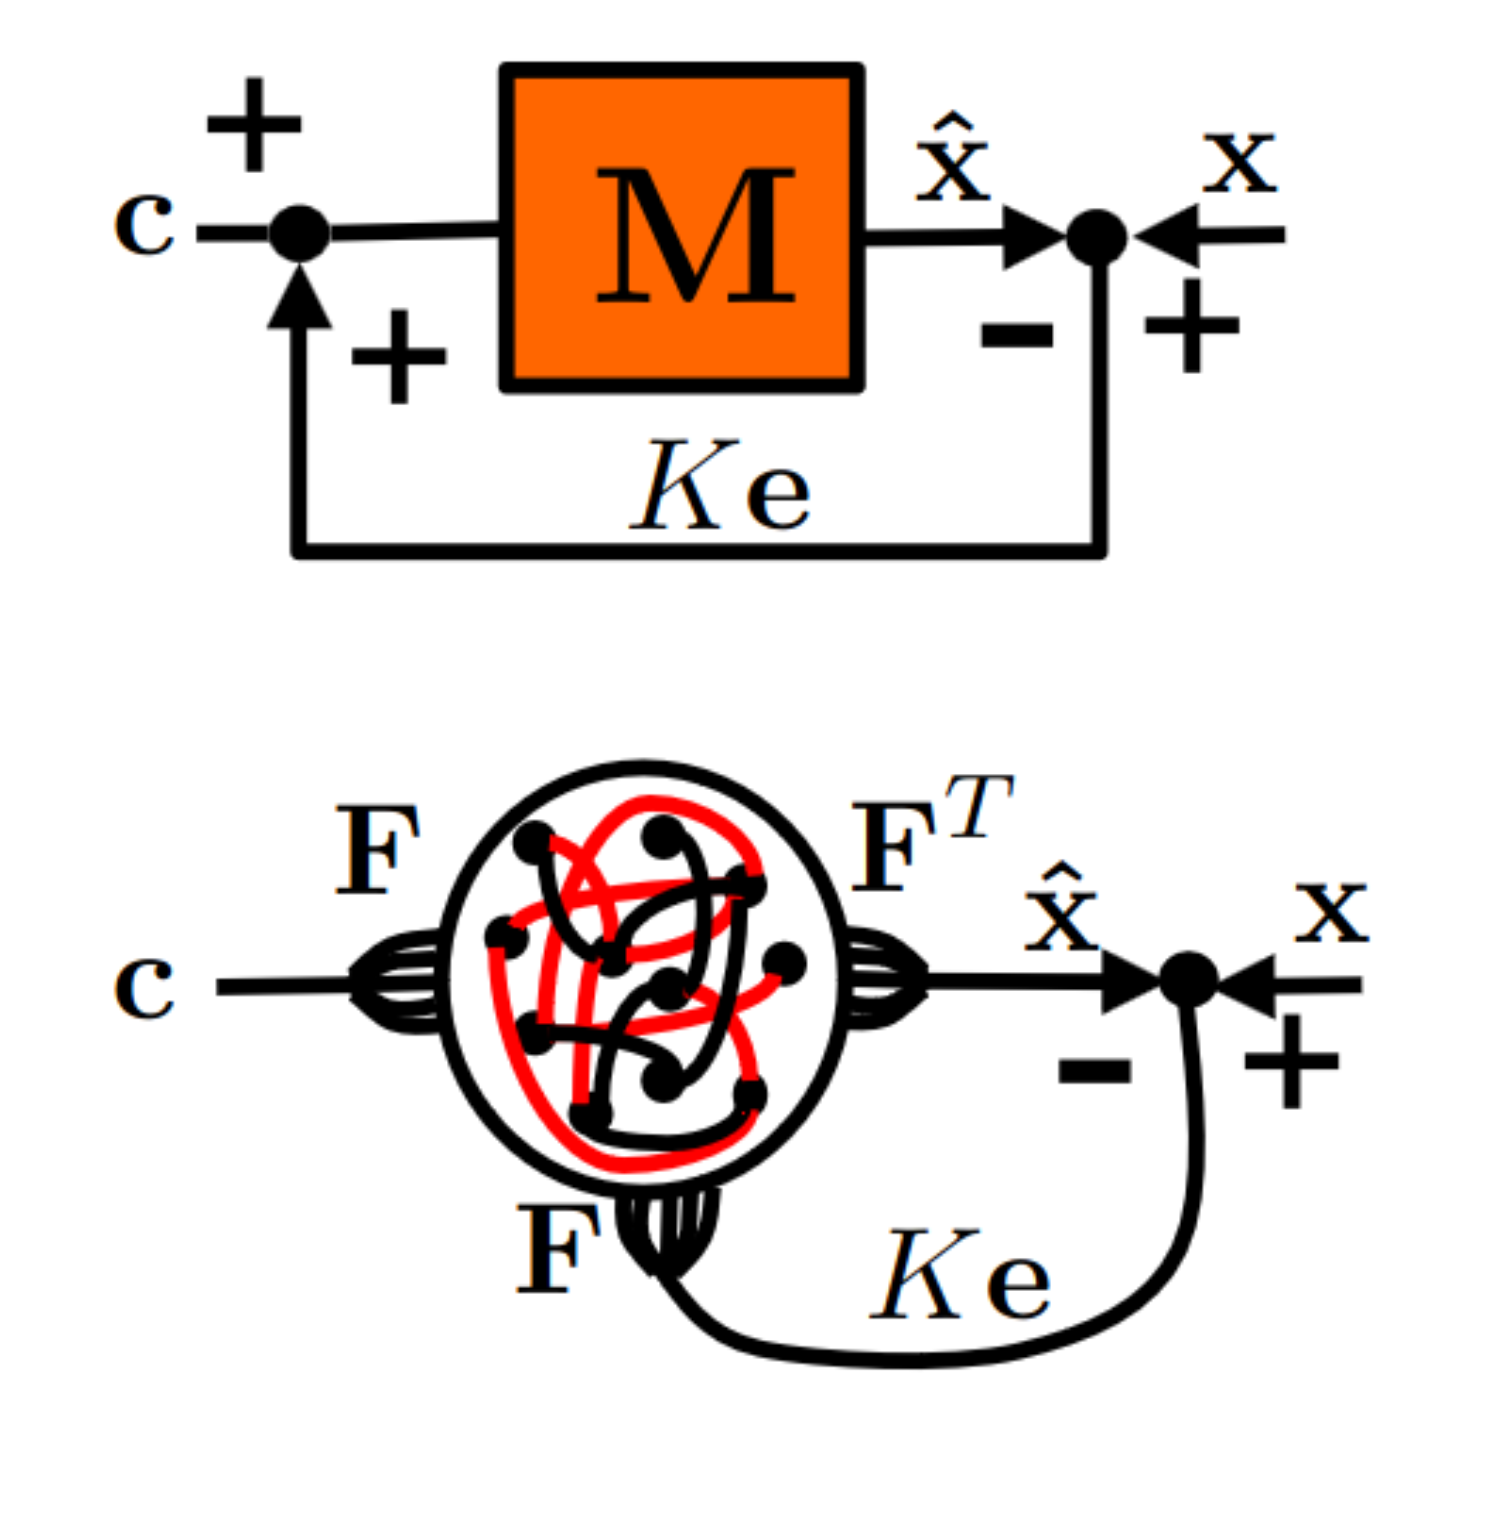
\includegraphics[width = 0.8\textwidth,trim= 0cm 0cm 0cm 8cm]{figures/slow_learning_rule.png}
			\end{figure}
			\begin{textblock*}{10pt}(300pt,240pt)
				\small
				\cite{bourdoukan_enforcing_2015}
			\end{textblock*}
		\end{column}
		\begin{column}{0.45\textwidth}
			Online Teacher-Student Scheme for $M$ under $\dot{x} = Mx +c$\\
			Matrix update under squared loss
			\begin{equation}
				\delta M \propto e\hat{x}^T \longrightarrow\delta W^s \propto F^T \left(e\hat{x}^T\right)F \approx F^T er
			\end{equation}
		\end{column}
	\end{columns}
\end{frame}

\begin{frame}{Fast Learning rule}


	\begin{textblock*}{10pt}(550pt,20pt)
		\small
		\begin{equation*}
		\begin{aligned}
		\dot{\hat{x}}=&(M-K \mathbf{I}) \hat{x}+c+K x\\
		W^s =& F\left(A + \lambda_d\mathbf{I}\right)F^T
		\end{aligned}
		\end{equation*}
	\end{textblock*}

	\begin{columns}
		\begin{column}{0.45\textwidth}
			\begin{figure}
				\centering
				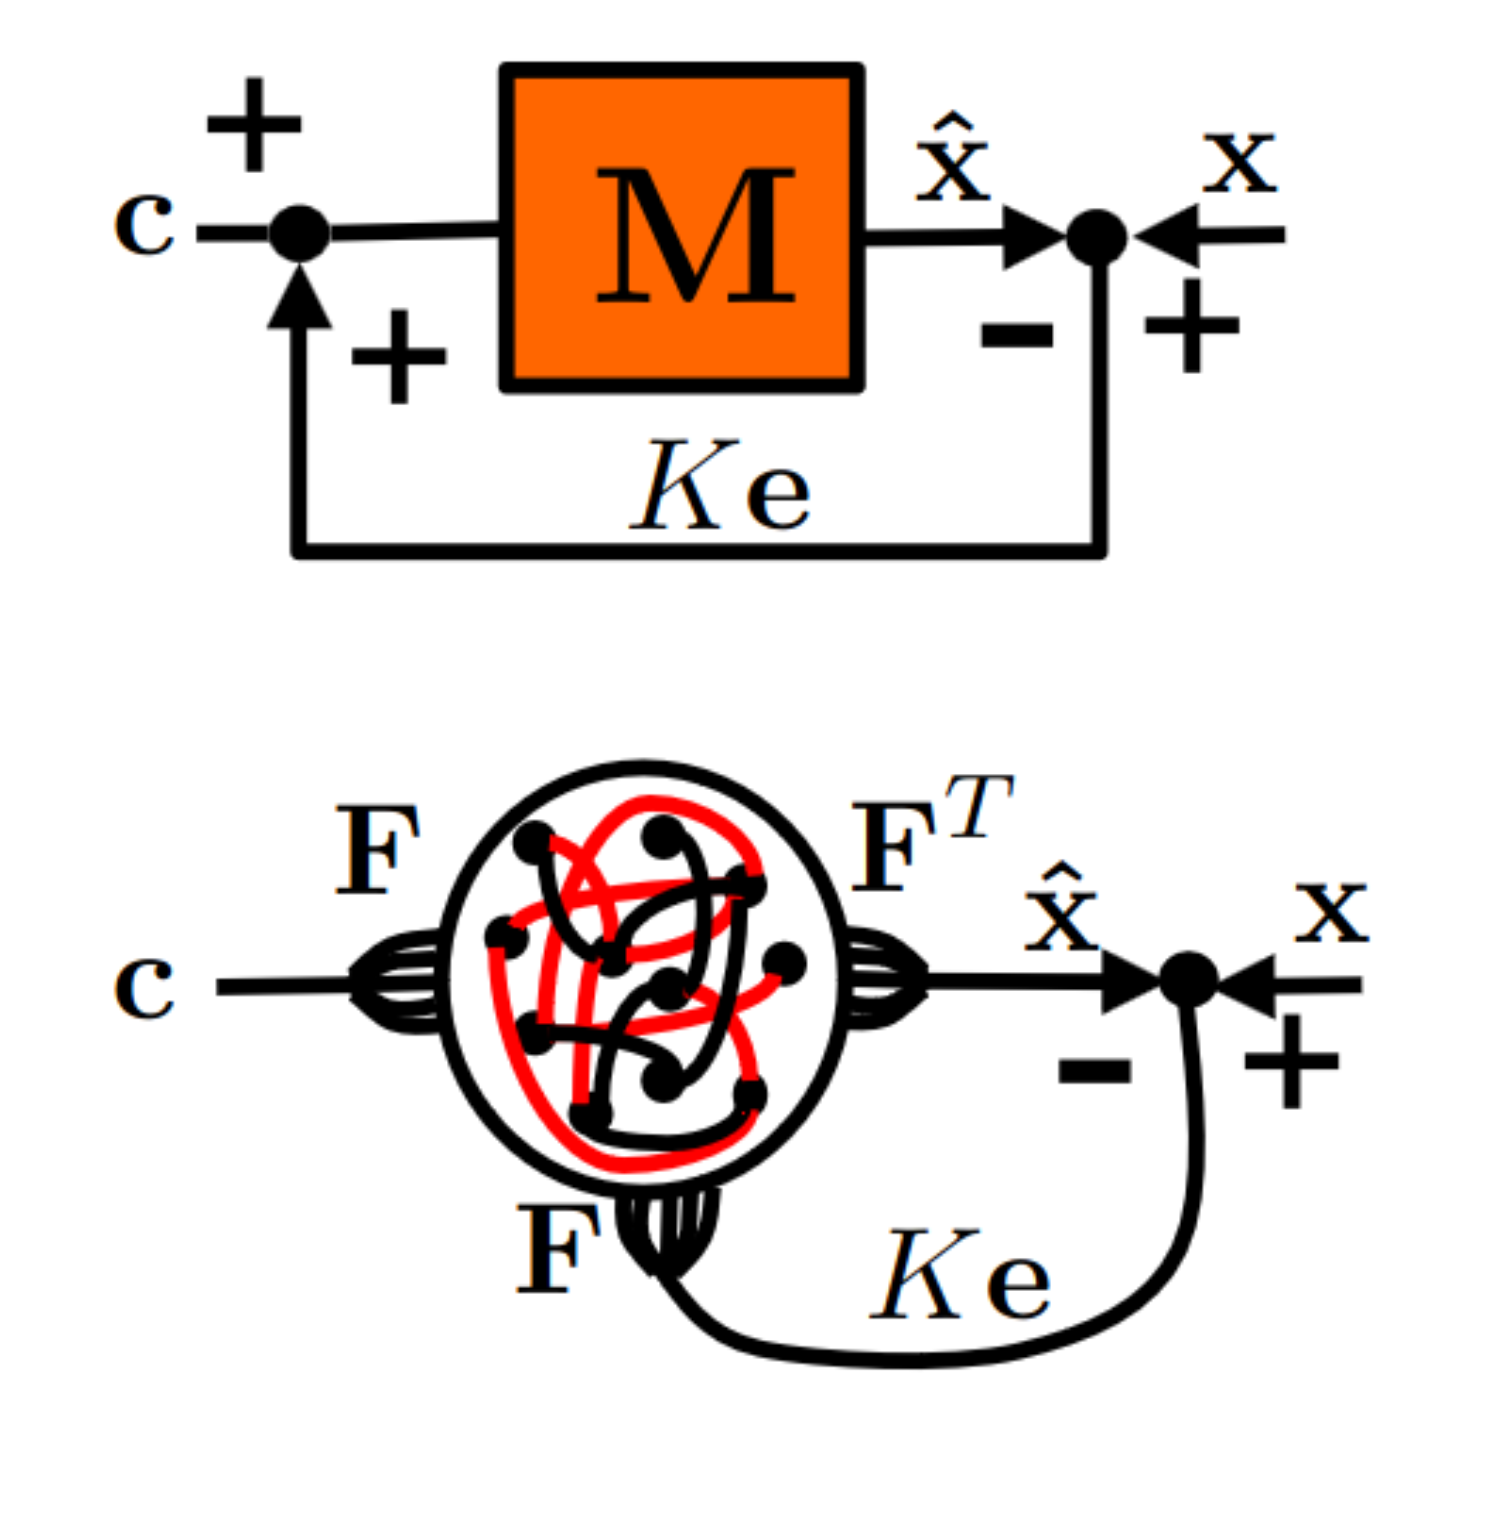
\includegraphics[width = 0.8\textwidth,trim= 0cm 0cm 0cm 8cm]{figures/slow_learning_rule.png}
			\end{figure}
			\begin{textblock*}{10pt}(300pt,240pt)
				\small
				\cite{bourdoukan_enforcing_2015}
			\end{textblock*}
		\end{column}
		\begin{column}{0.45\textwidth}
			Online Teacher-Student Scheme for $M$ under $\dot{x} = Mx +c$\\
			Matrix update under squared loss
			\begin{equation}
			\delta M \propto e\hat{x}^T \longrightarrow\delta W^s \propto F^T \left(e\hat{x}^T\right)F \approx F^T er
			\end{equation}
		\end{column}
	\end{columns}
\end{frame}

%\section{Learned Control}\insertsectionpage



%\section{Conclusion}\insertsectionpage
\begin{frame}{Conclusion}
	\begin{columns}
		\begin{column}{0.45\textwidth}
			\begin{itemize}
				\setlength\itemsep{1.0em}
				\item Very limited applicability
				\item Open loop + rank condition limiting factor
				\item Too inaccurate learning of slow weights $W^s$
				\item Too dependent on initial conditions in learning
			\end{itemize}
		\end{column}
		\vrule
		\begin{column}{0.45\textwidth}
			\begin{itemize}
				\setlength\itemsep{1.0em}
				\item In ideal conditions useable results achievable
				\item Only of theoretical interest
				\item Impressive accuracy
				\item Results are somewhat translatable to NEF and LSMs
			\end{itemize}
		\end{column}
	\end{columns}
\end{frame}

\insertendpage
\end{document}